\chapter{Unitary Renormalization Group Method}\label{urgform}
The URG method was introduced and formalised in refs.~\cite{anirbanurg1,anirbanurg2,anirbanmott1,anirbanmott2}.  This section is adapted from those references and expanded wherever required.
\section{Formalism and Results}
\subsection{Description of the problem}
We are given a Hamiltonian \(\mathcal{H}\) which is not completely diagonal in the occupation number basis of the electrons, \(\hat n_k\): \(\left[\mathcal{H},n_k\right] \neq 0\). \(k\) labels any set of quantum numbers depending on the system. For spin-less Fermions it can be the momentum of the particle, while for spin-full Fermions it can be the set of momentum and spin. There are terms that scatter electrons from one quantum number \(k\) to another quantum number \(k^\prime\).

We take a general Hamiltonian,
\begin{equation}\begin{aligned}
	\mathcal{H} = H_e \hat n_{q\beta} + H_h \left(1 - \hat n_{q\beta}\right) + c^\dagger_{q\beta}T + T^\dagger c_{q\beta}
\end{aligned}\end{equation}
Formally, we can decompose the entire Hamiltonian in the subspace of the electron we want to decouple (\(q\beta\)).
\begin{equation}\begin{aligned}
	\label{matham}
\mathcal{H} = \bordermatrix{~ & \ket{1} & \ket{0} \cr
              & H_1 & T \cr
              & T^\dagger & H_0 \cr}
\end{aligned}\end{equation}
The basis in which this matrix is written is \(\left\{\ket{1},\ket{0}\right\}\) where \(\ket{i}\) is the set of all states where \(\hat n_{q\beta}=i\). The aim of one step of the URG is to find a unitary transformation \(U\) such that the new Hamiltonian \(U \mathcal{H} U^\dagger\) is diagonal in this already-chosen basis.
\begin{equation}\begin{aligned}
	\tilde{\mathcal{H}} \equiv U \mathcal{H} U^\dagger = \bordermatrix{~ & \ket{1} & \ket{0} \cr
              & \tilde H_1 & 0 \cr
              & 0 & \tilde H_0 \cr}
\end{aligned}\end{equation}
\(U_q\) is defined by
\begin{equation}\begin{aligned}
	\tilde{\mathcal{H}} = U_q \mathcal{H} U^\dagger_q \text{   such that  } \left[\tilde{\mathcal{H}},n_q\right] = 0
\end{aligned}\end{equation}
It is clear that \(U\) is the diagonalizing matrix for \(\mathcal{H}\). Hence we can frame this problem as an eigenvalue equation as well. Let \(\ket{\psi_1},\ket{\psi_0}\) be the basis in which the original Hamiltonian \(\mathcal{H}\) has no off-diagonal terms corresponding to \(q\beta\). Hence, we can write
\begin{equation}\begin{aligned}
	\label{diageq}
    \mathcal{H} \ket{\psi_i} = \tilde H_i\ket{\psi_i}, i\in\left\{0,1\right\}
\end{aligned}\end{equation}
Since \(\ket{\psi_i}\) is the set of eigenstates of \(\mathcal{H}\) and \(\ket{i}\) is the set of eigenstates in which \(U\mathcal{H} U^\dagger\) has no off-diagonal terms corresponding to \(q\beta\), we can relate \(\ket{\psi_i}\) and \(\ket{i}\) by the same transformation : \(\ket{\psi_i} = U^\dagger\ket{i}\). We can expand the state \(\ket{\psi_i}\) in the subspace of \(q\beta\):
\begin{equation}\begin{aligned}
	\label{matpsi}
\ket{\psi_i} = \sum_{j=0,1} \ket{j}\bra{j}\ket{\psi_i} \equiv \ket{1}\ket{\phi_1^i} + \ket{0}\ket{\phi_0^i}\end{aligned}\end{equation}
where \(\ket{\phi_j^i} = \bra{j}\ket{\psi_i}\). If we substitute the expansion \ref{matham} into the eigenvalue equation \ref{diageq}, we get
\begin{equation}\begin{aligned}
	\left[H_e \hat n_{q\beta} + H_h \left(1 - \hat n_{q\beta}\right) + c^\dagger_{q\beta}T + T^\dagger c_{q\beta}\right]\ket{\psi_i} = \tilde H_i\ket{\psi_i}
\end{aligned}\end{equation}
The diagonal parts \(H_e = \text{tr}\left[\mathcal{H} \hat n_{q\beta}\right]\) and \(H_e = \text{tr}\left[\mathcal{H} \left(1 - \hat n_{q\beta}\right)\right]\) can be separated into a purely diagonal part \(\mathcal{H}^d\) that contains the single-particle energies and the multi-particle correlation energies or Hartree-like contributions, and an off-diagonal part  \(\mathcal{H}^i\) that scatters between the remaining degrees of freedom \(k\sigma \neq q\beta\). That is,
\begin{equation*}
\begin{gathered}
	H_e \hat n_{q\beta} + H_h \left(1 - \hat n_{q\beta}\right) = \mathcal{H}^d + \mathcal{H}^i\\
\end{gathered}
\end{equation*}
This gives
\begin{equation}\begin{aligned}
	\left[c^\dagger_{q\beta}T + T^\dagger c_{q\beta}\right]\ket{\psi_i} = \left(\tilde H_i - \mathcal{H}^i - \mathcal{H}^d\right)\ket{\psi_i}
\end{aligned}\end{equation}
\subsection{Obtaining the decoupling transformation}
We now define a new operator \(\hat \omega_i = \tilde H_i - \mathcal{H}^i\), such that 
\begin{equation}\begin{aligned}
	\left[c^\dagger_{q\beta}T + T^\dagger c_{q\beta}\right]\ket{\psi_i} = \left(\hat \omega_i - \mathcal{H}^d\right)\ket{\psi_i}
\end{aligned}\end{equation}
From the definition of \(\hat \omega_i\), we can see that it is Hermitian and has no term that scatters in the subspace of \(q\beta\), so it is diagonal in \(q\beta\) and we can expand it as \(\hat \omega_i = \hat \omega_i^1 \hat n_{q\beta} + \hat \omega_i^0 \left(1 - \hat n_{q\beta}\right)\). Using the expansion \ref{matpsi}, we can write
\begin{equation}\begin{aligned}
\hat \omega_i \ket{\psi_i} = \hat \omega_i^1 \ket{1}\ket{\phi_1^i} + \hat \omega_i^0 \ket{0}\ket{\phi_0^i}
\end{aligned}\end{equation}
Since the only requirement on \(\ket{\psi_i}\) is that it diagonalize the Hamiltonian in the subspace of \(q\beta\), there is freedom in the choice of this state. We can exploit this freedom and choose the \(\ket{\phi_{0,}^i}\) to be an eigenstates of \(\hat \omega_i^{1,0}\) corresponding to real eigenvalues \(\omega_i^{1,0}\):
\begin{equation}\begin{aligned}
	\left[\mathcal{H}^d + c^\dagger_{q\beta}T + T^\dagger c_{q\beta}\right]\ket{\psi_i(\omega_i)} = \left(\omega_i^1 - \mathcal{H}^d\right)\ket{1}\ket{\phi_1^i} + \left(\omega_i^0 - \mathcal{H}^d\right)\ket{0}\ket{\phi_0^i}
\end{aligned}\end{equation}
If we now substitue the expansion \ref{matpsi} and gather the terms that result in \(\hat n_{q\beta}=1\), we get
\begin{equation}\begin{aligned}
	\label{changea}
	c^\dagger_{q\beta}T\ket{0}\ket{\phi_0^i} = \left(\omega_i^1 - \mathcal{H}^d\right)\ket{1}\ket{\phi_1^i}
\end{aligned}\end{equation}
Similarly, gathering the terms that result in \(\hat n_{q\beta}=0\) gives
\begin{equation}\begin{aligned}
	\label{changeb}
	T^\dagger c_{q\beta}\ket{1}\ket{\phi_1^i} = \left(\omega_i^0 - \mathcal{H}^d\right)\ket{0}\ket{\phi_0^i}
\end{aligned}\end{equation}
We now define two many-particle transition operators:
\begin{equation}\begin{aligned}
	\label{etadefine}
{\eta}^\dagger(\omega_i^1) = \frac{1}{\omega_i^1- \mathcal{H}^d}c^\dagger_{q\beta}T \equiv G_1 c^\dagger_{q\beta}T\\
\eta(\omega_i^0) = \frac{1}{\omega_i^0- \mathcal{H}^d}T^\dagger c_{q\beta} \equiv G_0 T^\dagger c_{q\beta}
\end{aligned}\end{equation}
wher \(G_j\) is the propagator \(\frac{1}{\omega_i^j- \mathcal{H}^d}\). We can write this compactly as
\begin{equation}\begin{aligned}
	\label{etadagdef}
\eta(\hat \omega) = GT^\dagger c_{q\beta} = \frac{1}{\hat \omega_i- \mathcal{H}^d}T^\dagger c_{q\beta}
\end{aligned}\end{equation}
where \(\hat \omega_i = \omega_i^0\left(1 - \hat n_{q\beta}\right) + \omega_i^1\hat n_{q\beta} = \begin{pmatrix} \omega_i^1 & \\ & \omega_i^0 \end{pmatrix}\) is a 2x2 matrix and \(\mathcal{H}^d = \mathcal{H}^d_0\left(1 - \hat n_{q\beta}\right) + \mathcal{H}^d_1\hat n_{q\beta}\) and \(G = \left(\hat \omega - \mathcal{H}^d\right)^{-1}\). It is easy to check that this reproduces the previous forms of \(\eta_0\) and \(\eta_1^\dagger\).
We will later find that it is important to demand that these two be Hermitian conjugates of each other; that constraint is imposed on the denominators:
\begin{equation}\begin{aligned}
	\label{constraint}
\eta^\dagger(\omega_i^0) = \eta^\dagger(\omega_i^1) \implies \frac{1}{\omega_i^1- \mathcal{H}^d}c^\dagger_{q\beta}T = c^\dagger_{q\beta}T\frac{1}{\omega_i^0- \mathcal{H}^d}
\end{aligned}\end{equation}
Henceforth we will assume that this constraint has been imposed. 
\\\\In terms of these operators, eq.~\ref{changeb} becomes
\begin{equation}\begin{aligned}
    \ket{1}\ket{\phi_1^i} &= {\eta}^\dagger\ket{0}\ket{\phi_0^i}\\
    \ket{0}\ket{\phi_0^i} &= \eta\ket{1}\ket{\phi_1^i}
\end{aligned}\end{equation}
These allow us to write
\begin{equation}\begin{aligned}
	\label{trans}
	\ket{\psi_1} &= \ket{1}\ket{\phi_1^i} + \ket{0}\ket{\phi_0^i} = \left(1 + \eta\right)\ket{1}\ket{\phi_1^i}\\
	\ket{\psi_0} &= \left(1 + {\eta}^\dagger\right)\ket{0}\ket{\phi_0^i}
\end{aligned}\end{equation}
Recalling that \(\ket{\psi_i} = U^\dagger \ket{i}\), we can read off the required transformation:
\begin{equation}\begin{aligned}
	\label{Ui}
    U_1 &= 1 + \eta
\end{aligned}\end{equation}

\begin{figure}[htpb]
\begin{center}
	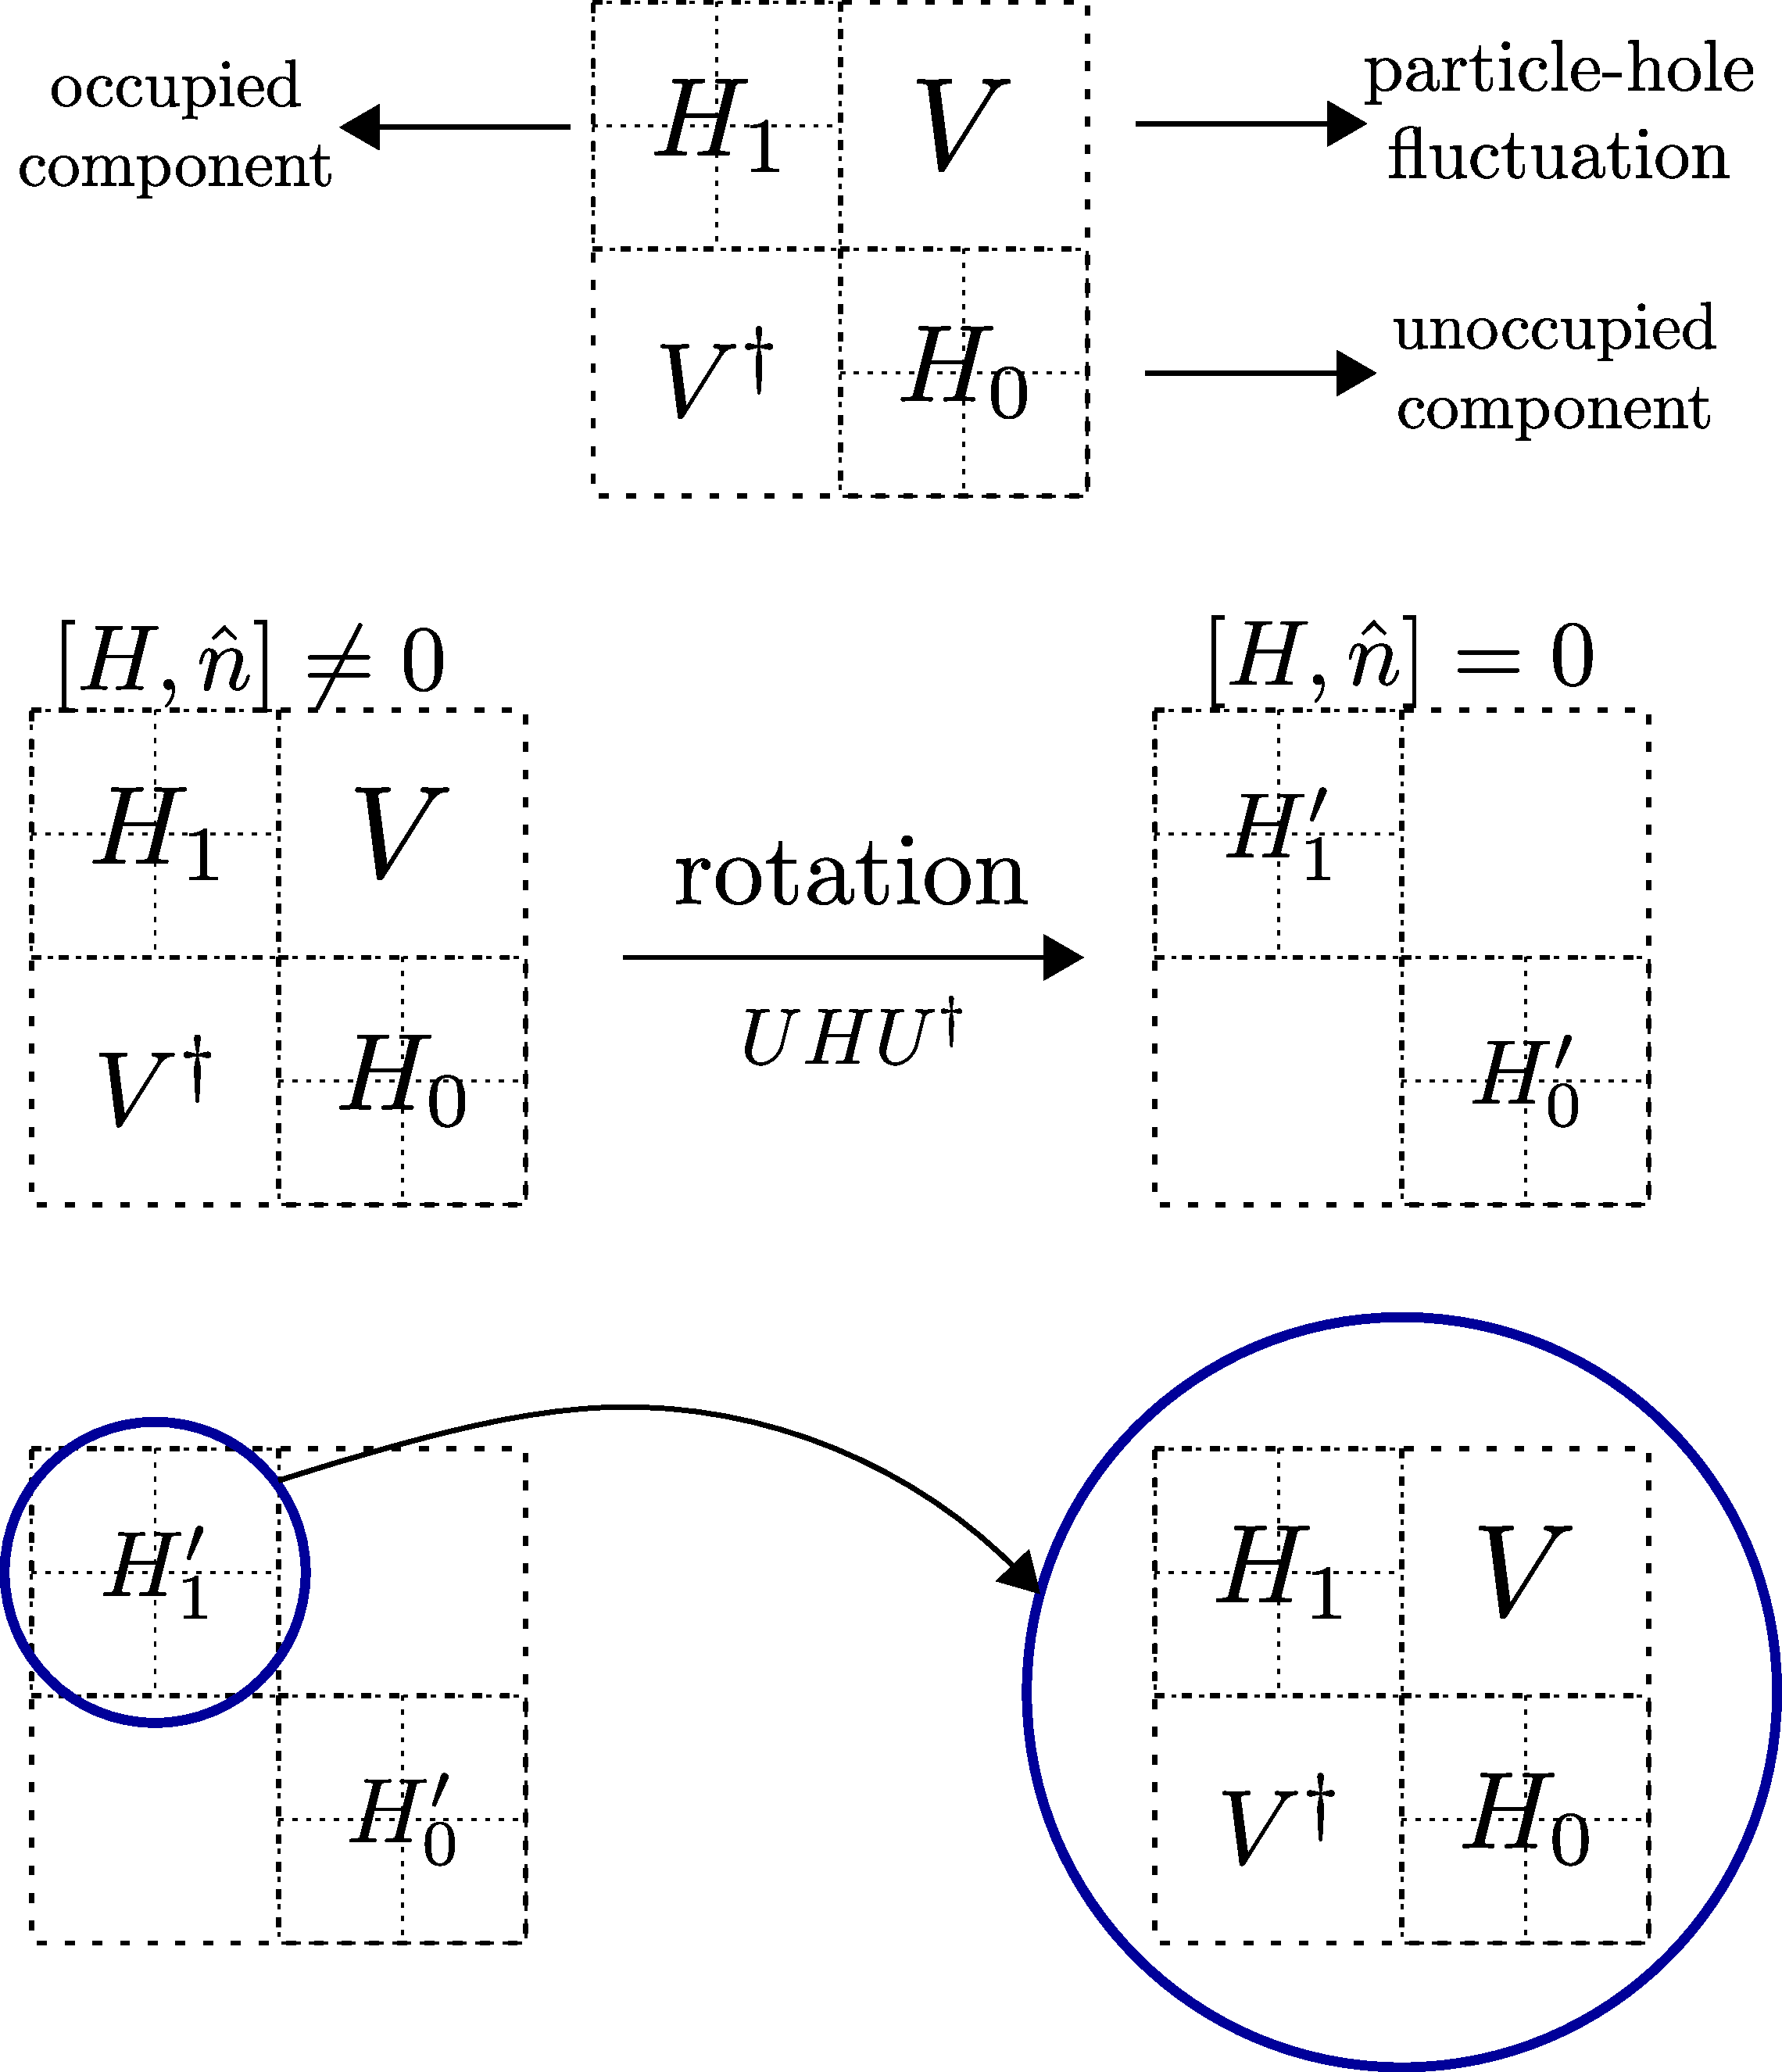
\includegraphics[width=0.6\textwidth]{../figures/URG_method.pdf}
\caption{Three steps of the URG: Decompose the Hamiltonian in a \(2\times 2\) matrix, apply the unitary operator to rotate it, then repeat these steps with one of the rotated blocks.}
\end{center}
\end{figure}

\subsection{Properties of the many-body transition operators}
The operators \(\eta\) have some important properties. First is the Fermionic nature:
\begin{equation}\begin{aligned}
	\eta^2 = {\eta^\dagger}^2 = 0 &&\left[{c^\dagger}^2 = c^2 = 0\right]\\
\end{aligned}\end{equation}
Second is:
\begin{equation}\begin{aligned}
	\label{antic}
    \ket{1}\ket{\phi_1^i} &= {\eta}^\dagger\ket{0}\ket{\phi_0^i} = \eta^\dagger \eta \ket{1}\ket{\phi_1^i} \implies \eta^\dagger \eta = \hat n_{q\beta}\\
    \ket{0}\ket{\phi_0^i} &= \eta\ket{1}\ket{\phi_1^i} = \eta \eta^\dagger\ket{\phi_0^i}\implies \eta  \eta^\dagger= 1 - \hat n_{q\beta}
\end{aligned}\end{equation}
and hence the anticommutator
\begin{equation}\begin{aligned}
	\label{antico}
    \implies \left\{\eta,\eta^\dagger\right\} = 1
\end{aligned}\end{equation}
Note that the three equations in \ref{antic} work only when applied on the eigenstate \(\ket{\psi_i}\) and not any arbitrary state.
\begin{equation*}
    \begin{gathered}
    \eta^\dagger \eta \ket{\psi_i} = \ket{1}\ket{\phi_1^i} = \hat n_{q\beta}\ket{\psi_i}\\
    \eta\eta^\dagger \ket{\psi_i} = \ket{0}\ket{\phi_0^i} = \left(1 - \hat n_{q\beta}\right)\ket{\psi_i}\\
    \left\{\eta^\dagger,\eta\right\}\ket{\psi_i} = \ket{\psi_i}
\end{gathered}
\end{equation*}
\subsection{Form of the unitary operators}\label{unitary-form}
Although we have found the correct similarity transformations \(U_i\) (eqs. \ref{Ui}), we need to convert them into a unitary transformation. Say we are trying to rotate the eigenstate \(\ket{\psi_1}\) into the state \(\ket{1}\). We can then work with the transformation
\begin{equation}\begin{aligned}
U_1 = 1 + \eta
\end{aligned}\end{equation}
In this form, this transformation is not unitary. It can however be written in an exponential form:
\begin{equation}\begin{aligned}
U_1 = e^{\eta}
\end{aligned}\end{equation}
using the fact that \(\eta^2 = 0\). It is shown in ref.~\cite{suzuki} that corresponding to a similarity transformation \(e^\omega\),there exists a unitary transformation \(e^G\) where
\begin{equation}\begin{aligned}
	G = \tanh^{-1}\left(\omega - \omega^\dagger\right)
\end{aligned}\end{equation}
Applying that to the problem at hand gives
\begin{equation}\begin{aligned}
	U_1^\dagger &= \exp\left\{\tanh^{-1}\left(\eta - \eta^\dagger\right)\right\}
 \end{aligned}\end{equation}
Let \(x = \tanh y\). Then,
\begin{equation}\begin{aligned}
x = \frac{e^{2y} + 1}{e^{2y} - 1} \implies y = \frac{1}{2} \log\frac{1+x}{1-x} \implies e^y = e^{\tanh^{-1}x} = \sqrt\frac{1+x}{1-x}
\end{aligned}\end{equation}
Therefore,
\begin{equation}\begin{aligned}
	\exp\left\{\tanh^{-1}\left(\eta - \eta^\dagger\right)\right\} &= \frac{1 + \eta - \eta^\dagger}{\sqrt{\left(1 + \eta^\dagger - \eta\right)\left(1 - \eta^\dagger + \eta\right)}}\\
                     &= \frac{1 + \eta - \eta^\dagger}{\sqrt{1 + \left\{\eta,\eta^\dagger\right\}}}\\
		     &= \frac{1}{\sqrt 2}\left(1 + \eta - \eta^\dagger\right)
\end{aligned}\end{equation}
The \textit{unitary} operator that transforms the entangled eigenstate \(\ket{\psi_1}\) to the state \(\ket{1}\) is thus
\begin{equation}\begin{aligned}
	\label{finalu}
	U_1 = \frac{1}{\sqrt 2}\left(1 + \eta^\dagger - \eta\right)
\end{aligned}\end{equation}
It can also be written as \(\exp\left\{\frac{\pi}{4}\left(\eta^\dagger - \eta\right)\right\}\) because
\begin{equation}\begin{aligned}
	\exp\left\{\frac{\pi}{4}\left(\eta^\dagger - \eta\right)\right\} &= 1 + \left(\eta^\dagger - \eta\right)\frac{\pi}{4} + \frac{1}{2!}\left(\eta^\dagger - \eta\right)^2\left(\frac{\pi}{4}\right)^2 + \frac{1}{3!}\left(\eta^\dagger - \eta\right)^3\left(\frac{\pi}{4}\right)^3 + ...\\
							   &= 1 + \left(\eta^\dagger - \eta\right)\frac{\pi}{4} - \frac{1}{2!}\left(\frac{\pi}{4}\right)^2 - \frac{1}{3!}\left(\eta^\dagger - \eta\right)\left(\frac{\pi}{4}\right)^3 + \frac{1}{4!}\left(\frac{\pi}{4}\right)^4 + ...\\
							   &= \cos \frac{\pi}{4} + \left(\eta^\dagger - \eta\right)\sin\frac{\pi}{4}\\
							   &= \frac{1}{\sqrt 2}\left(1 + \eta^\dagger - \eta\right)
\end{aligned}\end{equation}
There we used
\begin{equation}\begin{aligned}
	\left(\eta^\dagger - \eta\right)^2 = {\eta^\dagger}^2 + \eta^2 - \left\{\eta^\dagger,\eta\right\} = -1 &&\left[\because\eta^2 = {\eta^\dagger}^2=0\right]
\end{aligned}\end{equation}
and hence
\begin{equation}\begin{aligned}
	\left(\eta^\dagger - \eta\right)^3 = -1\left(\eta^\dagger - \eta\right)
\end{aligned}\end{equation}
and so on.
\subsection{Effective Hamiltonian}
We can now compute the form of the effective Hamiltonian that comes about when we apply \(U_1\) - that is - when we rotate one exact eigenstate \(\ket{\psi_1}\) into the occupied Fock space basis \(\ket{1}\). From eq.~\ref{finalu},
\begin{equation}\begin{aligned}
	U_1 \mathcal{H} U_1^\dagger &= \frac{1}{2}\left(1+\eta^\dagger - \eta\right)\mathcal{H}\left(1 + \eta - \eta^\dagger\right)\\
				    &= \frac{1}{2}\left(1+\eta^\dagger - \eta\right)\left(\mathcal{H} + \mathcal{H}\eta - \mathcal{H}\eta^\dagger\right)\\
				    &=\frac{1}{2}\left(\mathcal{H}+ \mathcal{H}\eta - \mathcal{H}\eta^\dagger + \eta^\dagger \mathcal{H} + \eta^\dagger\mathcal{H}\eta - \eta^\dagger \mathcal{H}\eta^\dagger - \eta\mathcal{H} - \eta \mathcal{H} \eta + \eta \mathcal{H} \eta^\dagger\right)\\
				    &=\frac{1}{2}\left(\mathcal{H}^d + \mathcal{H}^i + \mathcal{H}^I + \mathcal{H}\eta - \mathcal{H}\eta^\dagger + \eta^\dagger \mathcal{H} + \eta^\dagger\mathcal{H}\eta - \eta^\dagger \mathcal{H}\eta^\dagger - \eta\mathcal{H} - \eta \mathcal{H} \eta + \eta \mathcal{H} \eta^\dagger\right)\\
				    &=\frac{1}{2}\left(\mathcal{H}^d + \mathcal{H}^i + \mathcal{H}^I + \left[\eta^\dagger - \eta,\mathcal{H}\right] + \eta^\dagger\mathcal{H}\eta - \eta^\dagger \mathcal{H}\eta^\dagger - \eta \mathcal{H} \eta + \eta \mathcal{H} \eta^\dagger\right)\\
\end{aligned}\end{equation}
In the last two lines, we expanded the Hamiltonian into the three parts \(\mathcal{H}^d,\mathcal{H}^i\) and a third piece \(\mathcal{H}^I \equiv c_{q\beta}^\dagger T + T^\dagger c_{q\beta}\).
\\\\For reasons that will become apparent, we will split the terms into two groups:
\begin{equation}\begin{aligned}
	\tilde{\mathcal{H}} &= \frac{1}{2}\left(\underbrace{\mathcal{H}^d + \mathcal{H}^i + \left[\eta^\dagger - \eta,\mathcal{H}\right] + \eta^\dagger\mathcal{H}\eta + \eta \mathcal{H} \eta^\dagger}_\text{group 1} + \overbrace{\mathcal{H}^I - \eta^\dagger \mathcal{H}\eta^\dagger - \eta \mathcal{H} \eta}^\text{group 2}\right)\\
\end{aligned}\end{equation}
Group 2 can be easily shown to be 0. Note that terms that have two \(\eta\) or two \(\eta^\dagger\) sandwiching a \(\mathcal{H}\) can only be nonzero if the intervening \(\mathcal{H}\) has an odd number of creation or destruction operators.
\begin{equation}\begin{aligned}
	\label{beats}
\eta \mathcal{H} \eta = \eta c_q^\dagger  T \eta
\end{aligned}\end{equation}
and
\begin{equation}\begin{aligned}
	\label{tora}
\eta^\dagger \mathcal{H}\eta^\dagger = \eta^\dagger T^\dagger c_q \eta^\dagger
\end{aligned}\end{equation}
Group 2 becomes
\begin{equation}\begin{aligned}
	\label{group2}
\text{group 2} = \mathcal{H}^I - \eta^\dagger T^\dagger c_q \eta^\dagger - \eta c_q^\dagger  T \eta = c^\dagger_q T + T^\dagger c_q - \eta^\dagger T^\dagger c_q \eta^\dagger - \eta c_q^\dagger  T \eta
\end{aligned}\end{equation}
To simplify this, we use the relation
\begin{equation}\begin{aligned}
 \eta c_q^\dagger  T \eta &= \frac{1}{\omega_i^0 - \mathcal{H}^d}T^\dagger c_q c_q^\dagger  T \eta\\
			  &= T^\dagger c_q \frac{1}{\omega_i^1 - \mathcal{H}^d}c_q^\dagger  T \eta && \left[\text{eq.~\ref{constraint}}\right]\\
			  &= T^\dagger c_q \eta^\dagger\eta &&\left[\text{eq.~\ref{etadagdef}}\right]\\
			  &= T^\dagger c_q \hat n_q &&\left[\text{eq.~\ref{antic}}\right]
\end{aligned}\end{equation}
which gives
\begin{equation}\begin{aligned}
	\label{id1}
 \eta c_q^\dagger  T \eta  &= T^\dagger c_q 
\end{aligned}\end{equation}
Taking the Hermitian conjugate of eq.~\ref{id1} gives
\begin{equation}\begin{aligned}
	\label{id2}
\eta^\dagger T^\dagger c_q \eta^\dagger = c_q^\dagger T
\end{aligned}\end{equation}
Substituting the expressions \ref{id1} and \ref{id2} into the expression for group 2, \ref{group2}, shows that is vanishes. This leaves us only with group 1:
\begin{equation}\begin{aligned}
	\widetilde{\mathcal{H}} = \frac{1}{2}\left(\mathcal{H}^d + \mathcal{H}^i + \overbrace{\eta^\dagger\mathcal{H}\eta + \eta \mathcal{H} \eta^\dagger}^\text{group A} + \underbrace{\left[\eta^\dagger - \eta,\mathcal{H}\right]}_{group B}\right)
\end{aligned}\end{equation}
Group A simplifies in the following way. First note that \(\eta^\dagger \mathcal{H}^I \eta = \eta^\dagger \mathcal{H}^I \eta = 0\) must be 0 because it will involve consecutive \(c_{q\beta}\) or  consecutive \(c^\dagger_{q\beta}\). We are therefore left with the diagonal part of \(\mathcal{H}\), which is \(H_e \hat  n_{q\beta} + H_h \left(1 - \hat n_{q\beta}\right)\).
\begin{equation}\begin{aligned}
	\eta^\dagger\left[H_e \hat  n_{q\beta} + H_h \left(1 - \hat n_{q\beta}\right)\right]\eta + \eta\left[H_e \hat  n_{q\beta} + H_h \left(1 - \hat n_{q\beta}\right)\right]\eta^\dagger = \eta^\dagger H_h \eta + \eta H_e \eta^\dagger
\end{aligned}\end{equation}
This can be shown to be equal to the diagonal part:
\begin{equation}\begin{aligned}
	\text{group A} = \eta^\dagger H_h \eta + \eta H_e \eta^\dagger = H_e \hat n_{q\beta} + H_h\left(1 - \hat n_{q\beta}\right) = \mathcal{H}^d + \mathcal{H}^i
\end{aligned}\end{equation}
It can also be shown that
\begin{equation}\begin{aligned}
	\label{group B}
	\text{group B} = \left[\eta^\dagger - \eta,\mathcal{H}\right] = 2\left[c^\dagger_{q\beta} T,\eta\right]
\end{aligned}\end{equation}
Putting it all together,
\begin{equation}\begin{aligned}
	\label{final2}
	\tilde{\mathcal{H}}= \mathcal{H}^d + \mathcal{H}^i + \left[c^\dagger_{q\beta} T, \eta\right]
\end{aligned}\end{equation}
The renormalizing in the Hamiltonian is
\begin{equation}\begin{aligned}
	\Delta \mathcal{H} = \tilde{\mathcal{H}}- \mathcal{H}^d - \mathcal{H}^i = \left[c^\dagger_{q\beta} T, \eta\right]
\end{aligned}\end{equation}
Because of eq.~\ref{group B}, it can also be written as
\begin{equation}\begin{aligned}
	\label{renurg}
	\Delta \mathcal{H} = \frac{1}{2}\left[\eta^\dagger - \eta,\mathcal{H}_X\right] = \frac{1}{2}\left[\eta^\dagger - \eta,\mathcal{H}\right]
\end{aligned}\end{equation}
This form will be useful later when we make the connection with one-shot Schrieffer-Wolff transformation and CUT RG.

To check that the renormalised Hamiltonian indeed commutes with \(\hat n_{q\beta}\),
\begin{equation}\begin{aligned}
	\left[\widetilde{\mathcal{H}}, \hat n_{q\beta}\right] &= \left[\left[c_{q\beta}^\dagger T,\eta\right],\hat n_{q\beta}\right]\\
						      &=\left[c_{q\beta}^\dagger T \eta,\hat n_{q\beta}\right] - \left[\eta c_{q\beta}^\dagger T,\hat n_{q\beta}\right]\\
                   &=c^\dagger_{q\beta} T \eta \hat n_{q\beta} - \hat n_{q\beta}c^\dagger_{q\beta} T \eta &&\left[\text{2\textsuperscript{nd} [ .
		   ] is 0, }\because c_{q\beta}^\dagger \hat n_{q\beta} = \hat n_{q\beta} \eta=0\right]\\
                   &=c_{q\beta}^\dagger T \eta - c_{q\beta}^\dagger T \eta\\
             &=0
\end{aligned}\end{equation}
\subsection{Fixed point condition}\label{match}
Within the URG, it is a prescription that the fixed point is reached when the denominator of the RG equation vanishes. This is equivalent to either \(\omega_i^1 = \mathcal{H}^d_1 \) or \(\omega_i^0 = \mathcal{H}^d_0 \).
This shows that at the fixed point, one of the eigenvalues of \(\hat \omega_i\) matches the corresponding eigenvalue of the diagonal blocks. This also leads to the vanishing of the off-diagonal block, because eqs.~\ref{changea} and \ref{changeb} gives
\begin{equation}\begin{aligned}
	c^\dagger_{q\beta}T\ket{0}\ket{\phi_0^i} = \left(\omega_i^1 - \mathcal{H}^d_1\right)\ket{1}\ket{\phi_1^i} = 0 \implies c^\dagger_{q\beta}T = 0
\end{aligned}\end{equation}
\subsection{Multiple off-diagonal terms}
There is a subtle assumption in the definitions eq.~\ref{etadefine}. In order for \(\eta\) to be the Hermitian conjugate of \(\eta^\dagger\), \(\mathcal{H}_d\) cannot have any information that relates to the structure of \(T\). To see why, say the total off-diagonal term is composed of two parts: \(T = T_1 + T_2\).
\begin{equation}\begin{aligned}
	\eta &= \frac{1}{\omega_0 - \mathcal{H}_d}\left(T_1^\dagger + T_2^\dagger\right)c = \left[\frac{1}{\omega^0 - E^0_1} T_1^\dagger c+ \frac{1}{\omega^0 - E^0_2}T_2^\dagger c\right]\\
	\eta^\dagger &= \frac{1}{\omega^1 - \mathcal{H}_d}c^\dagger\left(T_1 + T_2\right) = \left[\frac{1}{\omega^1 - E^1_1}c^\dagger T_1 + \frac{1}{\omega^1 - E^1_2} c^\dagger T_2\right]\\
\end{aligned}\end{equation}
where \(\mathcal{H}_d T_i^\dagger c = E^0_i T_i^\dagger c\) and \(\mathcal{H}_d  c^\dagger T_i = E^1_i  c^\dagger T_i\). We can now see that in order for \(\eta = \left(\eta^\dagger\right)^\dagger\) to hold, two conditions must be met:
\begin{equation}\begin{aligned}
	\omega^0 - E_1^0 = \omega^1 - E_1^1, && \omega^0 - E_2^0 = \omega^1 - E_2^1
\end{aligned}\end{equation}
This will not hold generally. The correct solution is to realize that each such off-diagonal term \(T_i\) will come with its own quantum fluctuation scale \(\omega_i\).
\begin{equation}\begin{aligned}
	\eta &= \sum_i \frac{1}{\omega^0_i - E^0_i} T_i^\dagger c\\
	\eta^\dagger &= \sum_i \frac{1}{\omega^1_i - E^1_1}c^\dagger T_i
\end{aligned}\end{equation}
If we now impose the condition that \(\eta =  \left( \eta^\dagger \right) ^\dagger\), we get the relations
\begin{equation}\begin{aligned}
	\omega^0_i - \omega^1_i = E^0_i - E^1_1
\end{aligned}\end{equation}
and so
\begin{equation}\begin{aligned}
	\eta^\dagger - \eta &= \sum_i \frac{1}{\omega^0_i - E^0_i}\left(c^\dagger T_i - T_i^\dagger c\right)
\end{aligned}\end{equation}
The expression for the renormalization will not be just \(\left[c^\dagger T, \eta \right]\) in this case. That form will be non-Hermitian. The correct form is obtained from the more general form \(\left[\eta^\dagger - \eta, \mathcal{H}_X \right]\):
\begin{equation}\begin{aligned}
	\Delta \mathcal{H} &= \frac{1}{2}\left[\eta^\dagger - \eta, c^\dagger T + T^\dagger c\right]\\
		    &= \frac{1}{2}\sum_{ij} \frac{1}{\omega^0_i - E^0_i}\left[c^\dagger T_i - T_i^\dagger c, c^\dagger T_j + T_j^\dagger c\right]\\
		    &= \frac{1}{2}\sum_{ij} \frac{1}{\omega^0_i - E^0_i}\left[\hat n \left(T_i T_j^\dagger + T_j T_i^\dagger \right) - \left(1 - \hat n\right)\left(T_i^\dagger T_j + T_j^\dagger T_i\right)\right]\\
		    &= \frac{1}{2}\sum_{ij} \left(\frac{1}{\omega^0_i - E^0_i} + \frac{1}{\omega^0_j - E^0_j}\right)\left[\hat n T_i T_j^\dagger - \left(1 - \hat n\right)T_i^\dagger T_j\right]\\ 
\end{aligned}\end{equation}
\subsection{Equivalence of the two unitaries and preservation of partial trace}
In the subsection \ref{unitary-form}, we determined the form of the operator \(U_1\) that unitarily decouples the node \(q\beta\) from the other degrees of freedom. Eq.~\ref{finalu} was derived by reading off the transformation of \(\ket{1}\) to \(\ket{\psi_1}\), the first equation in \ref{trans}. We could easily have chosen the other equation in the same equation set,
\begin{gather*}
	\ket{\psi_0} = \left(1 + {\eta}^\dagger\right)\ket{0}\ket{\phi_0^i}
\end{gather*}
which gives a similarity  transformation \(1+\eta^\dagger\) and hence a unitary
\begin{equation}\begin{aligned}
	U_0 = \frac{1}{\sqrt 2}\left(1 + \eta - \eta^\dagger\right)
\end{aligned}\end{equation}
This \(\eta\) will however be different from the \(\eta\) in eq.~\ref{finalu}. The reason is, in order to get \(U_1\), we must start from the eigenvalue equation \(\mathcal{H} \ket{\psi_1} = \tilde H_1 \ket{\psi_1}\). This means that the corresponding \(\hat \omega\) will be defined as \(\hat \omega_1 = \tilde H_1 - \mathcal{H}^i\). On the other hand, in order to get \(U_0\) we must start with \(\mathcal{H} \ket{\psi_0} = \tilde H_0 \ket{\psi_0}\), and hence this \(\hat \omega\) will be \(\hat \omega_0 = \tilde H_0 - \mathcal{H}^i\). This difference in the \(\hat \omega\) will define two different sets of \(\eta\):
\begin{equation}\begin{aligned}
	\label{eta0}
\text{Starting from \(\ket{\psi_1}\):	}\eta_1 = \frac{1}{\omega_1^0- \mathcal{H}^d}T^\dagger c_{q\beta} && \text{and }\eta^\dagger_1 = \frac{1}{\omega_1^1- \mathcal{H}^d}T^\dagger c_{q\beta}\\
\text{Starting from \(\ket{\psi_0}\):	}\eta_0 = \frac{1}{\omega_0^0- \mathcal{H}^d}T^\dagger c_{q\beta} && \text{and }\eta^\dagger_0 = \frac{1}{\omega_0^1- \mathcal{H}^d}T^\dagger c_{q\beta}
\end{aligned}\end{equation}
The \(\omega_j^i\) eigenvalues have both upper and lower indices. The upper index \(i\) signifies which eigenstate it relates to - \(\omega_j \ket{i} = \omega_j^i\ket{i}\). The lower index refers to the exact eigenstate we started with - starting with \(\mathcal{H} \ket{\psi_j} = \tilde H_j\ket{\psi_j}\) leads to \(\omega_j\). The two unitaries are
\begin{equation}\begin{aligned}
	U_1 &= \frac{1}{\sqrt 2}\left(1 + \eta_1^\dagger - \eta_1\right)\\
	U_0 &= \frac{1}{\sqrt 2}\left(1 + \eta_0 - \eta_0^\dagger\right)
\end{aligned}\end{equation}
\\\\Since the two unitaries should give the same effective Hamiltonian, we require \(U_1 = U_0\). That requires \(\eta_1 = -\eta_0\). Comparing the expressions of the \(\eta\)s, we get
\begin{equation}\begin{aligned}
	\omega_1^0 - \mathcal{H}^d_0 = -\left(\omega_0^0 - \mathcal{H}^d_0\right)
\end{aligned}\end{equation}
This is the constraint that ensures that both unitaries give the same effective Hamiltonian. The condition \(\eta_1 + \eta_0 = 0\), when expressed without resolving \(\hat \omega\) into its eigenvalues can also be shown to be a statement of the preservation of the partial trace under the RG flow.
\begin{equation}\begin{aligned}
	\label{trace}
\eta_1 &= \frac{1}{\tilde H_1 - \mathcal{H}^i - \mathcal{H}^d}T^\dagger c_{q\beta}\\
\eta_0 &= \frac{1}{\tilde H_0 - \mathcal{H}^i - \mathcal{H}^d}T^\dagger c_{q\beta}\\
\implies  \eta_1 + \eta_0 &= \left[\frac{1}{\tilde H_1 - \mathcal{H}^i - \mathcal{H}^d} + \frac{1}{\tilde H_0 - \mathcal{H}^i - \mathcal{H}^d}\right]T^\dagger c_{q\beta} = 0\\
\implies \tilde H_1 - \mathcal{H}^i - \mathcal{H}^d &= -\left[\tilde H_0 - \mathcal{H}^i - \mathcal{H}^d\right]\\
\implies \tilde H_1 + \tilde H_0 &= 2\mathcal{H}_0
\end{aligned}\end{equation}
\(\mathcal{H}_0 = \mathcal{H}^i + \mathcal{H}^d\) is the total diagonal part of the bare model. To match the dimensions, we must take \(\tilde H_1 = E_1 \otimes I\) and similarly \(\tilde H_0 = E_0 \otimes I\), where the rotated Hamiltonian is
\begin{equation}\begin{aligned}
\tilde H = \begin{pmatrix} E_1 & 0 \\ 0 & E_0\end{pmatrix}
\end{aligned}\end{equation}
Therefore, the trace of the rotated Hamiltonian is \(t_\text{new} = E_1 + E_0 \). The trace of the LHS in the final equation of \ref{trace} is \(\text{tr}\left(\tilde H_1 + \tilde H_0\right) = \text{tr}\left(E_1 \otimes I + E_0 \otimes I\right) = 2\left(E_1 + E_0\right) = 2t_\text{new}\). The trace of the RHS in final equation of \ref{trace} is \(2\times\text{tr}\left(\mathcal{H}_0\right) = 2t_\text{old}\) where \(t_\text{old} = \text{tr}\left(\mathcal{H}_0\right)\) is the trace of the old Hamiltonian. Equating the LHS and RHS gives \(t_\text{new} = t_\text{old}\).

\subsection{Complete generator for the unitary transformation}
Given some operator \(O_0\), we can generate a family of unitarily-connected operators \(O_j\) using a unitary operator \(U(t)\):
\begin{equation}\begin{aligned}
	\label{familiy_O}
	O_j = U_j O(0) U_j^\dagger, ~ ~ j = 1,2,\ldots
\end{aligned}\end{equation}
The discrete change equation for \(O_j\) can be represented in the form of a commutator:
\begin{equation}\begin{aligned}
	\label{generator}
	\Delta O_j \equiv O_{j+1} - O_j = \left[O_j, S_j\right] 
\end{aligned}\end{equation}
where 
\begin{equation}\begin{aligned}
	S_j = U_j \Delta U^\dagger_j~.
\end{aligned}\end{equation}
Note that because \(\Delta \left( U_j U_j^\dagger \right) = 0\), we have \(\left(\Delta U_j\right) U_j^\dagger = -U_j\left(\Delta U_j^\dagger\right)\) and so \(S_j\) is anti-Hermitian. To verify that eq.~\ref{familiy_O} is indeed the solution of eq.~\ref{generator}, we differentiate eq.~\ref{familiy_O}:
\begin{equation}\begin{aligned}
	O_{j+1} - O_j = \Delta U_j O(0) U_j^\dagger + U_j O(0) \Delta U_j^\dagger = \Delta U_j U_j^\dagger O_j + O_j U_j \Delta U_j^\dagger = \left[O_j, S_j\right] 
\end{aligned}\end{equation}
This shows that given a family of operators eq.~\ref{familiy_O} connected through \(U_j\), we can obtain a generator \(S_j\) that defines the flow equation of \(O_j\).

Since the URG is unitary, we should be able to obtain such a generator for it as well. From the expression of the unitary transformation of URG:
\begin{equation}\begin{aligned}
	U_j = \frac{1}{\sqrt 2}\left( 1 + \eta_j^\dagger - \eta_j \right) 
\end{aligned}\end{equation}
From the definition of the generator \(S_j\), we then get
\begin{equation}\begin{aligned}
	S_j = \frac{1}{2}\left( 1 + \eta_j^\dagger - \eta_j \right) \left(\eta_{j+1} - \eta^\dagger_{j+1} - \eta_j + \eta^\dagger_{j}\right)
\end{aligned}\end{equation}
The operators \(\eta_j\) and its hermitean conjugate can be thought of as angular momentum creation and annihilation operators acting on the \(2\times 2\) Hilbert space of the occupied and vacant states \(\ket{1}\ket{\phi_{1}}, \ket{0}\ket{\phi_{0}}\):
\begin{align}
	\eta_j \ket{1}\ket{\phi_1} = \ket{0}\ket{\phi_{0}},~ ~\eta_j \ket{0}\ket{\phi_0} = 0, && \eta^\dagger_j \ket{0}\ket{\phi_{0}} = \ket{1}\ket{\phi_1},~ ~\eta^\dagger_j \ket{1}\ket{\phi_1} = 0,\\
\end{align}
To check whether they have the corect algebra, we design the three spin operators \(S^i, i=\{x,y,z\}\).
\begin{equation}\begin{aligned}
	S^x &= \frac{1}{2}\left(S^+ + S^-\right) = \frac{1}{2}\left(\eta^\dagger_j + \eta_j\right) \\
	S^y &= \frac{1}{2i}\left(S^+ - S^-\right) = \frac{1}{2i}\left(\eta^\dagger_j - \eta_j\right) \\
	S^z &= \hat n - \frac{1}{2}
\end{aligned}\end{equation}
The commutation relations give
\begin{equation}\begin{aligned}
	\left[S^x, S^y\right] &= \frac{1}{4i}\left[\eta^\dagger_j + \eta_j, \eta^\dagger_j - \eta_j\right] = \frac{1}{2i}\left[\eta_j, \eta_j^\dagger\right] = \frac{1}{2i}\left(1 - \hat n - \hat n\right) = \frac{-1}{i}\left(\hat n - \frac{1}{2}\right) = i S^z\\
	\left[S^y, S^z\right] &= \frac{1}{2i}\left[\eta^\dagger_j - \eta_j, \hat n - \frac{1}{2}\right] = \frac{1}{2i}\left[-\eta_j \hat n - \hat n \eta_j^\dagger\right] = \frac{1}{2i}\left(-\eta_j - \eta_j^\dagger\right) = \frac{i}{2}\left(\eta_j^\dagger + \eta_j\right)= i S^x\\
	\left[S^z, S^x\right] &= \frac{1}{2}\left[\hat n - \frac{1}{2}, \eta^\dagger_j + \eta_j\right] = \frac{1}{2}\left[\hat n \eta_j^\dagger - \eta_j\hat n \right] = \frac{1}{2}\left(\eta_j^\dagger - \eta_j\right) = i\frac{1}{2i}\left(\eta_j^\dagger - \eta_j\right) = i S^y\\
\end{aligned}\end{equation}
These operators therefore satisfy the commutation algebra of angular momentum operators \(\left[S^i, S^j\right] = i\epsilon^{ijk}S^k\).

\subsection{A note on the various quantum fluctuation scales \(\pmb\omega_i^j\)}
At a particular step of the URG, there are two quantum fluctuation energy scales associated with each sector. If we rotate \(\ket{\psi_1}\) to \(\ket{1}\) (particle/occupied sector), the corresponding unitary will be a function of \(\omega_1^{0,1}\). If we, on the other hand, rotate \(\ket{\psi_0}\) to \(\ket{0}\) (hole/unoccupied sector), the unitary will be a function of \(\omega_0^{0,1}\). The superscript \(j\) signifies whether this particular \(\omega_i^j\) is an eigenvalue corresponding to \(\ket{1,\phi_i}\) or \(\ket{0,\phi_i}\). \(\omega^0_i\) occurs in the many-body transition operator \(\eta\), because \(\eta\) is preceded by \(c\) and hence it picks out the eigenstate \(\ket{0,\phi_i}\). On the other hand, \(\omega^1_i\) occurs in the many-body transition operator \(\eta^\dagger\), because that is preceded by \(c^\dagger\). This constrains these two values, because we must have \(\eta(\omega_i^0) = \left(\eta^\dagger(\omega_i^1)\right)^\dagger\) (eq.~\ref{constraint}), for each value of \(i\), giving us two constraints in total. The subscript \(i\) signifies whether \(\omega_i^j\) is a part of the particle sector unitary \(U_1(\omega_1^j)\) or the hole sector unitary \(U_0(\omega_0^j)\). As mentioned in the previous section, since both ways are equivalent, we must have \(U_1 = U_0\) which leads to the constraints \(\eta(\omega_0^j) = -\eta(\omega_1^j)\). All the independent constraints are listed below.
\begin{equation}\begin{aligned}
	\label{omegarel}
\omega_1^0 - \omega_1^1 &=\mathcal{H}_d^0 - \mathcal{H}_d^1\\
\omega_0^0 - \omega_0^1 &= \mathcal{H}_d^0 - \mathcal{H}_d^1\\
\omega_1^0 + \omega_0^0 &= 2\mathcal{H}_d^0
\end{aligned}\end{equation}
The first two come from \(\eta(\omega_i^0) = \left(\eta^\dagger(\omega_i^1)\right)^\dagger\) while the last comes from \(\eta(\omega_0^j) = -\eta(\omega_1^j)\). These are the only independent relations. Other relations like the one between \(\omega_1^0\) and \(\omega_0^1\) can be derived from these. This means that we have four \(\omega\) and three constraints, such that each step of the URG is characterized by just a single independent quantum fluctuation scale.
\section{Prescription}
Given a Hamiltonian
\begin{equation}\begin{aligned}
\mathcal{H} = \mathcal{H}_1 + \mathcal{H}_0 + c^\dagger T + T^\dagger c
\end{aligned}\end{equation}
the goal is to look at the renormalization of the various couplings in the Hamiltonian as we decouple high energy electron states. Typically we have a shell of electrons at some energy \(D\). During the process, we make one simplification. We assume that there is only one electron on that shell at a time, say with quantum numbers \(q,\sigma\), and calculate the renormalization of the various couplings due to this electron. We then sum the momentum \(q\) over the shell and the spin \(\beta\), and this gives the total renormalization due to decoupling the entire shell. 
\\\\From eq.~\ref{final2}, the first two terms in the rotated Hamiltonian are just the diagonal parts of the bare Hamiltonian; they are unchanged in that part. The renormalization comes from the third term. For one electron \(q\beta\) on the shell, the renormalization is
\begin{equation}\begin{aligned}
	\Delta \mathcal{H} = \left[c_{q\beta}^\dagger \text{Tr}\left(\mathcal{H} c_{q\beta}\right),\eta\right] = c_{q\beta}^\dagger \text{Tr}\left(\mathcal{H} c_{q\beta}\right)\eta - \eta c_{q\beta}^\dagger \text{Tr}\left(\mathcal{H} c_{q\beta}\right)
\end{aligned}\end{equation}
Since this assumes we have obtained this from \(U_1\), it is fair to tag the \(\eta\) with a suitable label:
\begin{equation}\begin{aligned}
	\Delta \mathcal{H} = c_{q\beta}^\dagger \text{Tr}\left(\mathcal{H} c_{q\beta}\right)\eta_1 - \eta_1 c_{q\beta}^\dagger \text{Tr}\left(\mathcal{H} c_{q\beta}\right)
\end{aligned}\end{equation}
It is clear that the first term takes into account virtual excitations that start from a filled state (\(\hat n_{q\beta}=1\) initially) - such a term is said to be a part of the \textit{particle sector}.
\begin{equation}\begin{aligned}
	\Delta_1 \mathcal{H} = c_{q\beta}^\dagger \text{Tr}\left(\mathcal{H} c_{q\beta}\right)\eta_1
\end{aligned}\end{equation}
The second term, on the other hand, considers excitations that start from an empty state. They constitute the \textit{hole sector}.
\begin{equation}\begin{aligned}
	\Delta_0 \mathcal{H} = -\eta_1 c_{q\beta}^\dagger \text{Tr}\left(\mathcal{H} c_{q\beta}\right)
\end{aligned}\end{equation}
To write the total renormalization in a particle-hole symmetric form, we can use the relation \(\eta_0=-\eta_1\), such that both the terms will now come with a positive sign:
\begin{equation}\begin{aligned}
	\Delta \mathcal{H} = c_{q\beta}^\dagger \text{Tr}\left(\mathcal{H} c_{q\beta}\right)\eta_1 + \eta_0 c_{q\beta}^\dagger \text{Tr}\left(\mathcal{H} c_{q\beta}\right)
\end{aligned}\end{equation}
We can make one more manipulation: using eq.~\ref{constraint}, we get
\begin{equation}\begin{aligned}
	\Delta \mathcal{H} = c_{q\beta}^\dagger \text{Tr}\left(\mathcal{H} c_{q\beta}\right)\eta_1 + \text{Tr}\left(c_{q\beta}^\dagger \mathcal{H}\right) c_{q\beta}\eta^\dagger_0 
\end{aligned}\end{equation}
This form of the total renormalization is identical to the one we use in the "Poor Man's scaling"-type of renormalization that was used to get the scaling equations in the Kondo and Anderson models \cite{Anderson,haldane}. Writing down the forms of \(\eta\) and \(\eta^\dagger\) explicitly, we get
\begin{equation}\begin{aligned}
	\Delta \mathcal{H} = c_{q\beta}^\dagger \text{Tr}\left(\mathcal{H} c_{q\beta}\right)\frac{1}{\omega_1^0 - \mathcal{H}^d_0} \text{Tr}\left(c_{q\beta}^\dagger\mathcal{H}\right) c_{q\beta}+ \text{Tr}\left(c_{q\beta}^\dagger \mathcal{H}\right) c_{q\beta} \frac{1}{\omega_0^1 - \mathcal{H}^d_1}c_{q\beta}^\dagger\text{Tr}\left(\mathcal{H} c_{q\beta}\right)
\end{aligned}\end{equation}
The renormalization due to the entire shell is obtained by summing over all states on the shell.
\begin{equation}\begin{aligned}
	\label{delta}
	\Delta \mathcal{H} = \sum_{q\beta}\left[c_{q\beta}^\dagger \text{Tr}\left(\mathcal{H} c_{q\beta}\right)\frac{1}{\omega_1^0 - \mathcal{H}^d_0} \text{Tr}\left(c_{q\beta}^\dagger\mathcal{H}\right) c_{q\beta} + \text{Tr}\left(c_{q\beta}^\dagger \mathcal{H}\right) c_{q\beta}\frac{1}{\omega_0^1 - \mathcal{H}^d_1}c_{q\beta}^\dagger\text{Tr}\left(\mathcal{H} c_{q\beta}\right)\right] 
\end{aligned}\end{equation}
These equations will now need to be simplified. For example, in the particle sector, we can set \(\hat n_{q\beta}=0\) in the numerator, because there is no such excitation in the initial state. Similarly, in  the hole sector, we can set \(\hat n_{q\beta}=1\) because that state was occupied in the initial state. Another simplification we typically employ is that \(\mathcal{H}^d_{0,1}\) will, in general, have the energies of all the electrons. But we consider only the energy of the on-shell electrons in the denominator. After integrating out these electrons, we can rearrange the remaining operators to determine which term in the Hamiltonian it renormalizes and what is the renormalization.

At first sight, one might think that we must evaluate lots of traces to obtain the terms in \(\Delta \mathcal{H}\). A little thought reveals that the terms in the numerator are simply the off-diagonal terms in the Hamiltonian; \(\text{Tr}\left(c^\dagger_{q\beta}\mathcal{H} \right)c_{q\beta}\) is the off-diagonal term that has \(c_{q\beta}\) in it, and \(c_{q\beta}^\dagger \text{Tr}\left(\mathcal{H} c_{q\beta}\right)\) is the off-diagonal term that has \(c^\dagger_{q\beta}\) in it. \(\mathcal{H}^D\) is just the diagonal part of the Hamiltonian.
\section{URG analysis of the star graph model}
\noindent
\begin{minipage}{0.5\textwidth}
	The star graph problem has already been analyzed using URG and an extensive study of its entanglement properties has already been carried out, in ref.~\cite{spa_star}. Here we focus on just deriving the RG equations. The system consists of \(N\) spin-like degrees of freedom (labeled 1 through N) individually talking to a spin at the center (labeled 0). Each spin \(i\) (\(\in \left[0,N\right]\)) has an on-site energy \(\epsilon_i\). The coupling strength between 0 and \(i\) (\(\in \left[1,N\right]\)) is \(J_i\). We choose the on-site energies such that \(\epsilon_{i+1} > \epsilon_i, i\in\left[N-1,1\right]\). In this way, \(\epsilon_1\) is the infrared limit and \(\epsilon_N\) is the ultraviolet limit.
\begin{equation}\begin{aligned}
	\mathcal{H} = \epsilon_0 S^z_0 + \sum_{i=1}^N\left[\epsilon_i S^z_i + J_i \vec{S}_0 \cdot \vec{S}_i\right]
\end{aligned}\end{equation}
\end{minipage}
\hfill
\begin{minipage}{0.4\textwidth}
\begin{center}
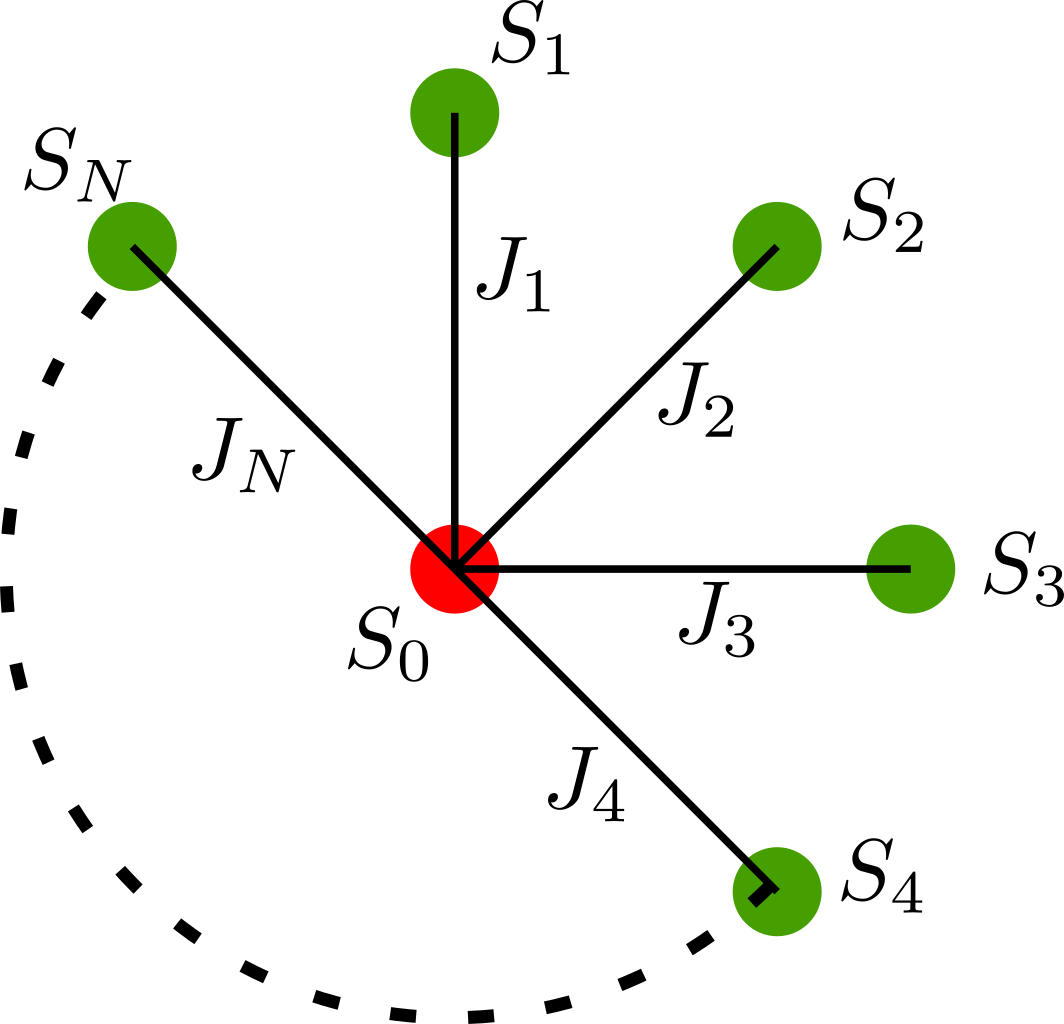
\includegraphics[width=0.8\textwidth]{../figures/stargraph_.png}
\captionof{figure}{Star Graph model}
\end{center}
\end{minipage}

By converting the last term into \(S^z\) and \(S^\pm\), we can write the Hamiltonian as
\begin{equation}\begin{aligned}
	\mathcal{H} = \epsilon_0 S^z_0 + \sum_{i=1}^N\left[\epsilon_i S^z_i + J_i\left(S^z_0 S^z_i + \frac{1}{2}\left(S_0^+ S^-_i + S_0^- S^+_i\right)\right)\right]
\end{aligned}\end{equation}

\subsection{Calculation of Renormalization}

The RG involves decoupling the nodes \(N\) through 1, and looking at the resultant renormalization in \(\epsilon_i\) and \(J_i\). As a simplification, we will ignore the lower nodes in the denominator and keep only the node currently being decoupled, ie node \(N\). Since node \(0\) is connected to node \(N\), we will keep node \(0\) in the denominator as well. Making this simplification gives
\begin{equation}\begin{aligned}
	\label{stardiag}
\mathcal{H}^D =\epsilon_0 S^z_0 + \epsilon_N S^z_N + J_NS^z_0 S^z_N 
\end{aligned}\end{equation}
The off-diagonal part in the subspace of the node \(N\) is
\begin{equation}\begin{aligned}
\mathcal{H}_X = S_N^+ T + T^\dagger S_N^- = \frac{1}{2}J_N \left(S_N^+ S_0^- + S_N^- S_0^+\right)
\end{aligned}\end{equation}
The renormalization on doing one step of the URG is given by
\begin{equation}\begin{aligned}
	\Delta \mathcal{H} &=  S_N^+ T \frac{1}{\omega_0^1 - \mathcal{H}^D}T^\dagger  S_N^- + T^\dagger  S_N^- \frac{1}{\omega_1^0 - \mathcal{H}^D} S_N^+ T\\
			   &= \frac{J_N^2}{4}S_N^+ S_0^- \frac{1}{\omega_0^1 - \epsilon_0 S^z_0 - \epsilon_N S^z_N - J_NS^z_0 S^z_N}S_0^+  S_N^- + \frac{J_N^2}{4}S_0^+  S_N^- \frac{1}{\omega_1^0 - \epsilon_0 S^z_0 - \epsilon_N S^z_N - J_NS^z_0 S^z_N} S_N^+ S_0^-
\end{aligned}\end{equation}
There, \(N\) refers to the spin being decoupled. The first Greens function has \(S_0^+\) and \(S_N^-\) in front of it, so we substitute \(S_0^z = \frac{1}{2}, S_N^z = -\frac{1}{2}\) in that Greens function. For the other Greens function we do the opposite.
\begin{equation}\begin{aligned}
	\Delta \mathcal{H} &= \frac{J_N^2}{4}S_N^+ S_0^- \frac{1}{\omega_1^0 - \frac{1}{2}\epsilon_0  + \frac{1}{2}\epsilon_N + \frac{1}{4}J_N}S_0^+  S_N^- + \frac{J_N^2}{4}S_0^+  S_N^- \frac{1}{\omega_0^1 + \frac{1}{2}\epsilon_0 - \frac{1}{2}\epsilon_N + \frac{1}{4}J_N} S_N^+ S_0^-
\end{aligned}\end{equation}

To relate \(\omega_1^0\) and \(\omega_0^1\), we use eq.~\ref{omegarel}:
\begin{equation}\begin{aligned}
	\omega_1^0 + \omega_0^1 = \mathcal{H}^D_0 + \mathcal{H}^D_1 = -\frac{1}{2}J_N \implies \omega_1^0 \equiv \omega, ~ ~\omega_0^1 \equiv \omega^\prime = -\frac{1}{2}J_N - \omega
\end{aligned}\end{equation}
So, the renormalization becomes
\begin{equation}
	\Delta \mathcal{H} = \frac{J_N^2}{4}\frac{1}{\omega - \frac{1}{2}\epsilon_0  + \frac{1}{2}\epsilon_N + \frac{1}{4}J_N}\left(S_N^+ S_0^- S_0^+  S_N^- - S_0^+  S_N^- S_N^+ S_0^-\right) = \frac{J_N^2}{4}\frac{1}{\omega - \frac{1}{2}\epsilon_0  + \frac{1}{2}\epsilon_N + \frac{1}{4}J_N}\left(S_N^z - S_0^z\right)
\end{equation}
There we used  \(S^+ S^- = \frac{1}{2} + S^z\) and \(S^- S^+ = \frac{1}{2} - S^z\).

We can now read off the renormalizations in \(\epsilon_N\) and \(\epsilon_0\).
\begin{equation}\begin{aligned}
	\Delta \epsilon_N &= \frac{1}{4}J_N^2 \frac{1}{\omega - \frac{1}{2}\epsilon_0 + \frac{1}{2}\epsilon_N + \frac{1}{4}J_N}\\
	\Delta \epsilon_0 &= -\frac{1}{4}J_N^2 \frac{1}{\omega - \frac{1}{2}\epsilon_0 + \frac{1}{2}\epsilon_N + \frac{1}{4}J_N}
\end{aligned}\end{equation}
\subsection{Nature of flows}
We are interested in looking at the renormalization of the central node energy \(\epsilon_0\), upon removing the nodes \(N\) through 1. We will hence concentrate on the second RG equation. We first make some simplifying assumptions: \(J_i = J, \epsilon_i = \epsilon\) for all \(i\in\{1,N\}\).
\begin{equation}\begin{aligned}
	\label{stareq}
	\Delta \epsilon_0 &= -\frac{1}{4}J^2 \frac{1}{\omega - \frac{1}{2}\epsilon_0 + \frac{1}{2}\epsilon + \frac{1}{4}J}
\end{aligned}\end{equation}
Define \(\tilde\omega = \omega + \frac{1}{2}\epsilon + \frac{1}{4}J\).
\begin{equation}\begin{aligned}
	\Delta \epsilon_0 &= -\frac{1}{4}J^2 \frac{1}{\tilde \omega - \frac{1}{2}\epsilon_0}
\end{aligned}\end{equation}
Our goal here is to look for a fixed-point condition such that the denominator vanishes at some point of the RG. If we start with a bare of \(\epsilon_0\) such that \(\tilde \omega - \frac{1}{2}\epsilon_0 > 0\), the denominator will be positive and the RG equation will be irrelevant. This means that \(\epsilon_0\) will keep on decreasing, and the denominator will keep on becoming more and more positive, meaning there cannot be a fixed point in this situation.

If, on other hand, we start with a bare of \(\epsilon_0\) such that \(\tilde \omega - \frac{1}{2}\epsilon_0 < 0\), the denominator will be negative and the RG equation will be relevant. This means that \(\epsilon_0\) will keep on increasing, and the denominator will keep on becoming more and more negative, meaning there cannot be a fixed point in this situation either. These situations are depicted in figure \ref{star1}.
\begin{figure}
	\centering
	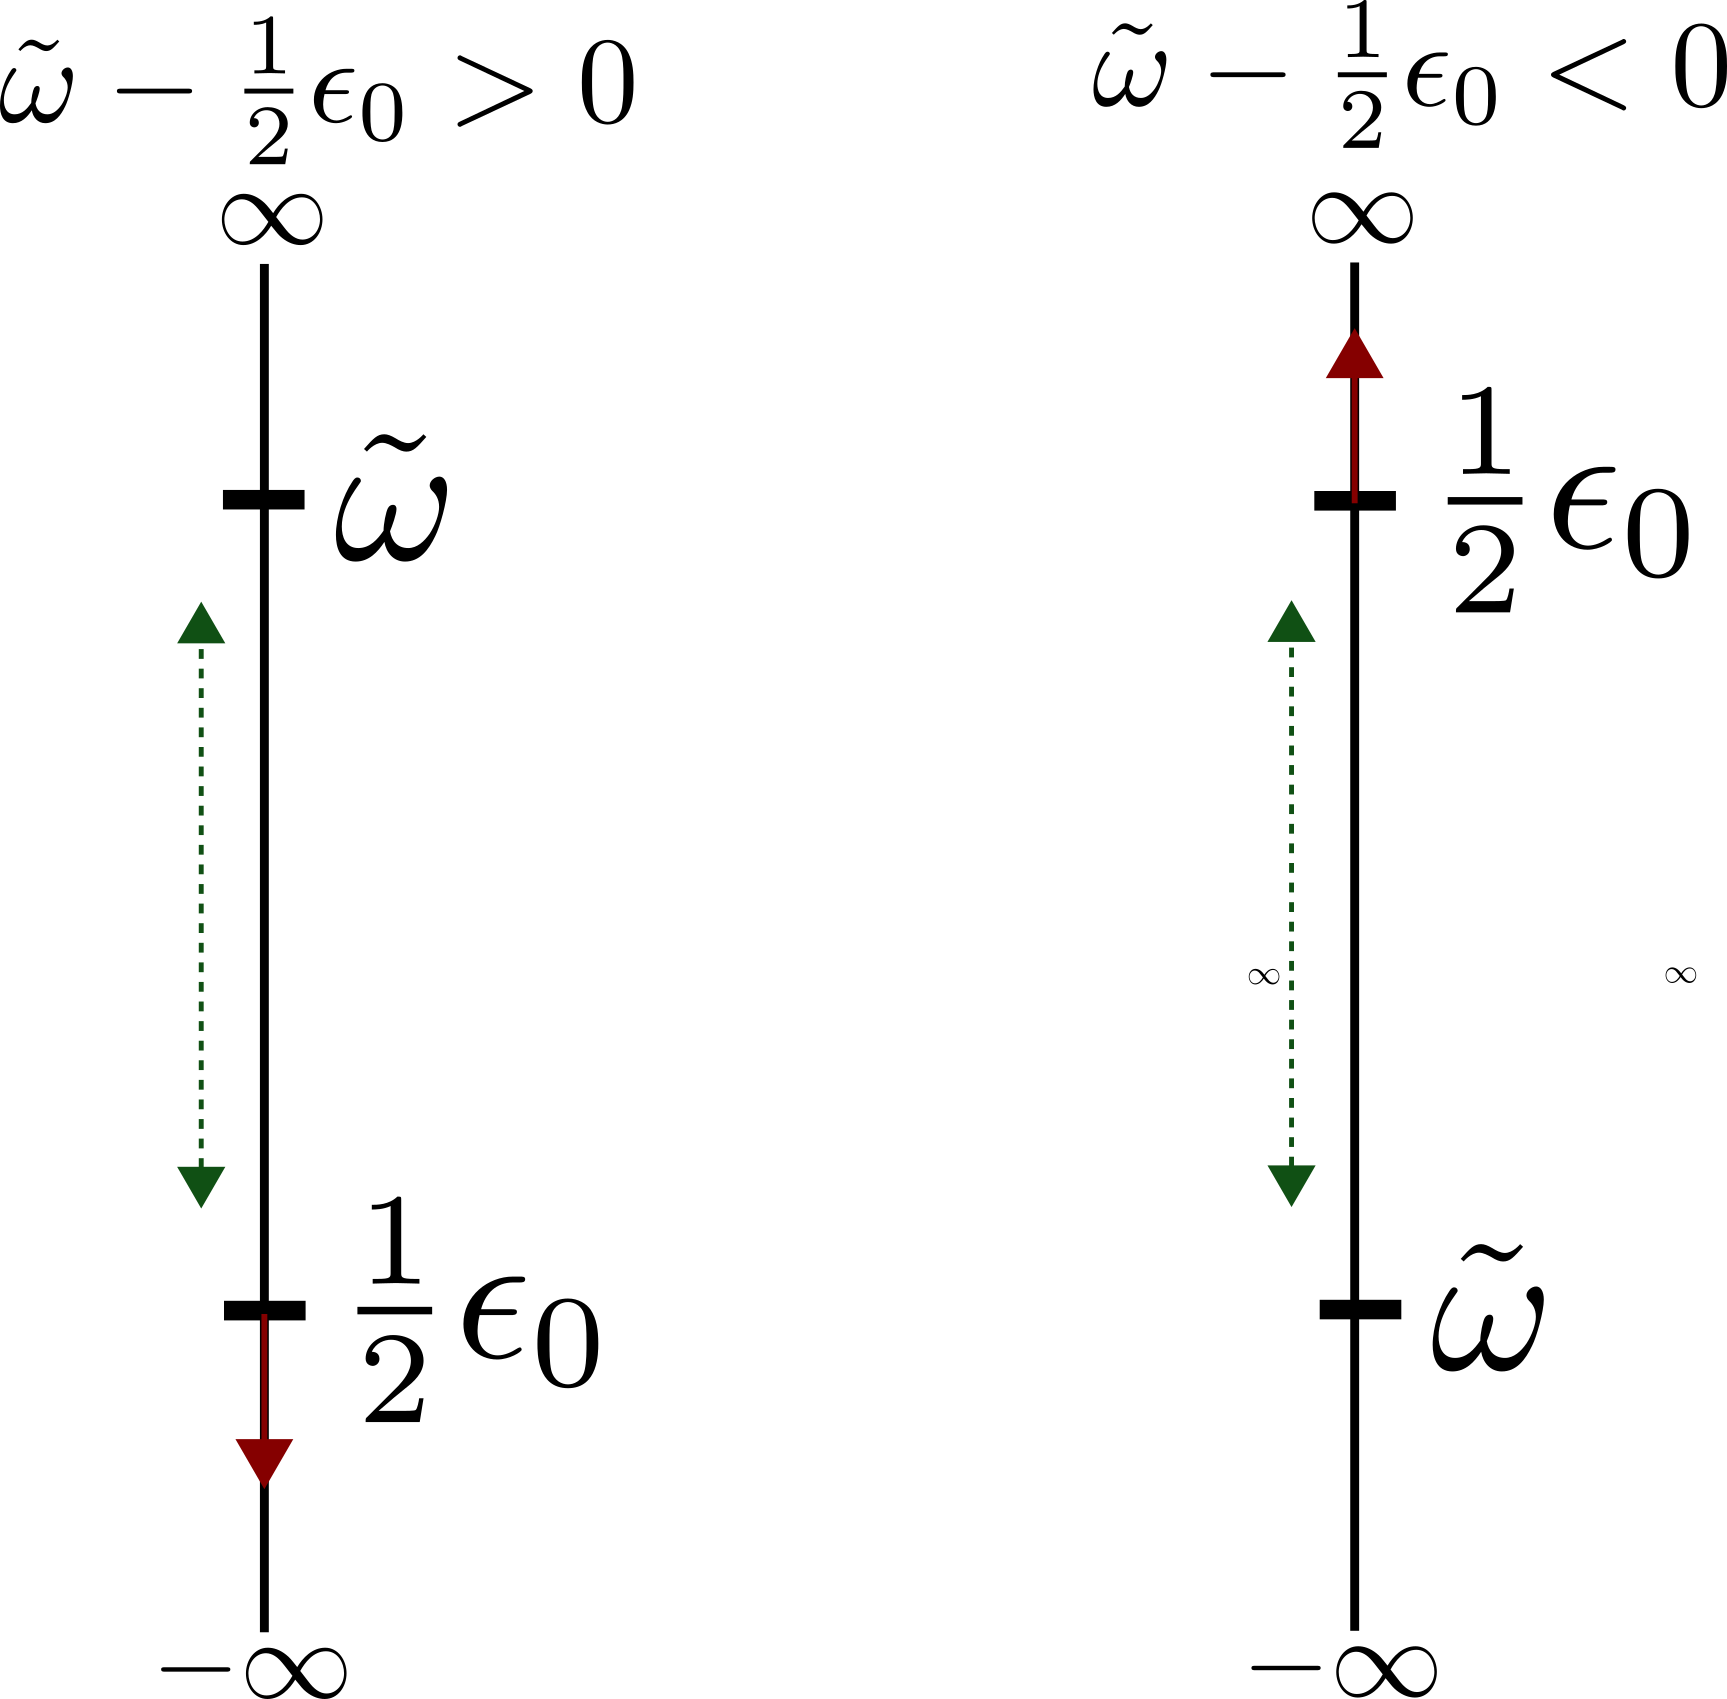
\includegraphics[scale=0.35]{star}
	\hfill
	\vline
	\hfill
	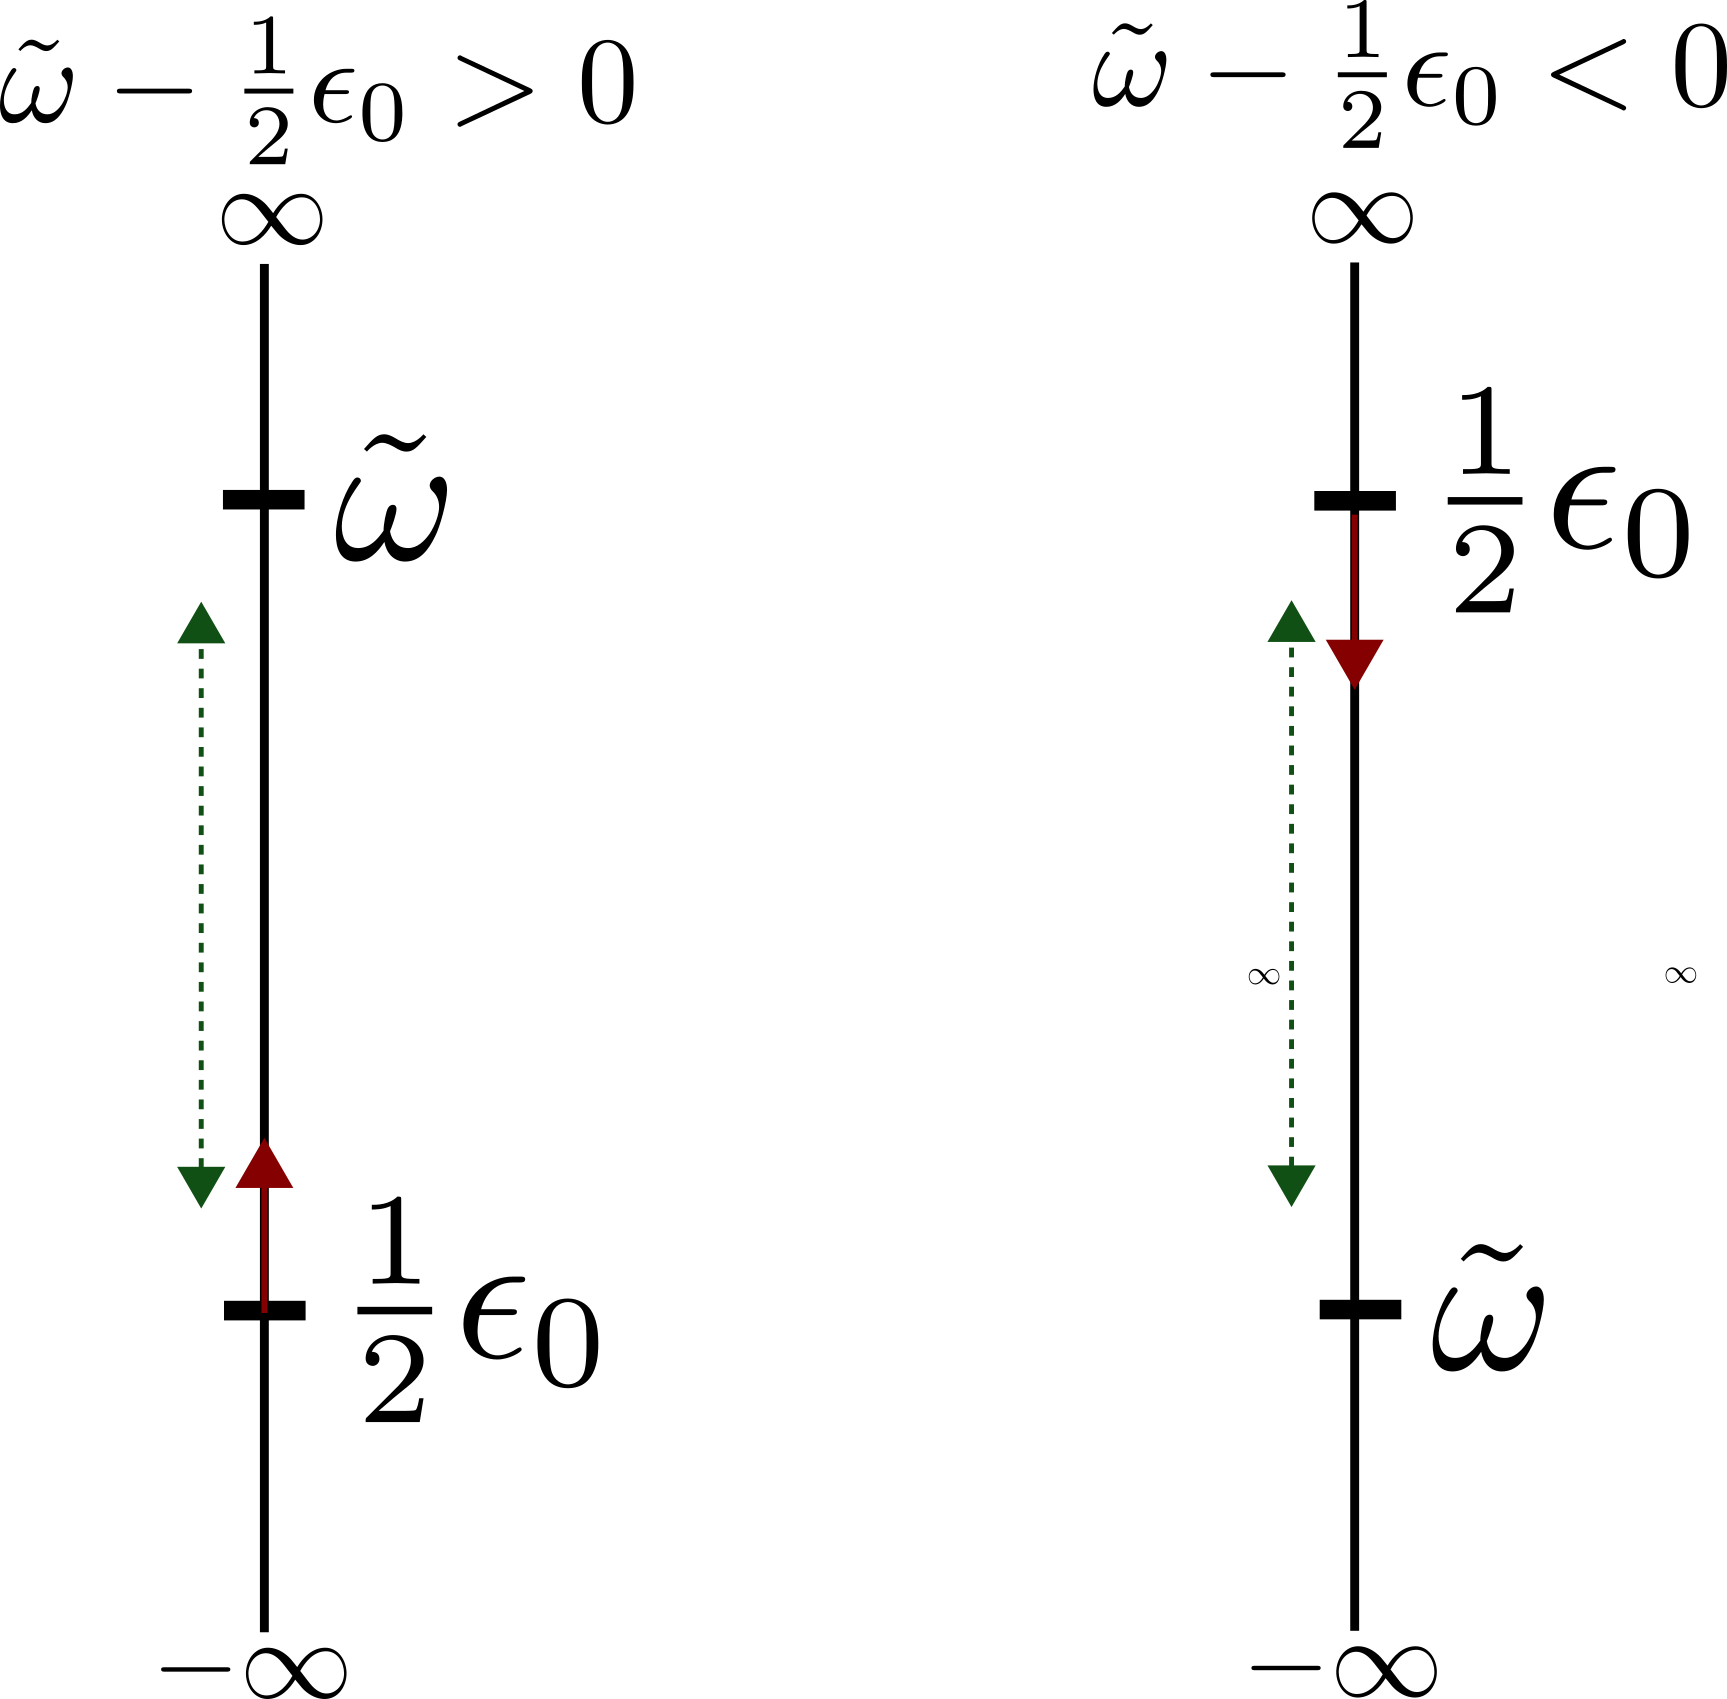
\includegraphics[scale=0.35]{star3}
	\caption{Left: RG flow for the two cases. The green line is the distance between the bare values of the two couplings, and hence also the magnitude of the denominator. The red arrow denotes the direction in which \(\epsilon_0\) will flow. Upward flow is increase. In both cases, the flow is such that the distance between the two quantities (and hence the magnitude of the denominator) increases. The RG fixed point occurs when the magnitude of the denominator goes to 0. This happens if the distance vanishes. Since the distance necessarily increases, we cannot get a fixed point in this way. Right: RG flow for the two cases with the new \(-\tilde \omega = \omega^\prime - \frac{1}{2}\epsilon + \frac{1}{4}J\). Now we can see that in both cases, the flow is such that the distance (green dotted line) between the couplings decreases. A fixed point is reached when this distance vanishes.}
	\label{star1}
\end{figure}

Since we cannot find a fixed point, we will use a different \(\omega\). Instead of \(\omega_1^0\), we will use \(\omega_1^1\). From eq.~\ref{omegarel}, we have 
\begin{equation}\begin{aligned}
	\omega_1^0  - \omega_1^1 = \mathcal{H}^D_0 - \mathcal{H}^D_1 = \epsilon_0 - \epsilon_N = \epsilon_0 - \epsilon
\end{aligned}\end{equation}
Defining \(\omega_1^1 = \omega^\prime\) and substituting this in eq.~\ref{stareq} gives
\begin{equation}\begin{aligned}
	\Delta \epsilon_0 = -\frac{1}{4}J^2 \frac{1}{\omega^\prime - \frac{1}{2}\epsilon + \frac{1}{2}\epsilon_0 + \frac{1}{4}J}
\end{aligned}\end{equation}
We again define \(-\tilde \omega = \omega^\prime - \frac{1}{2}\epsilon + \frac{1}{4}J\).
\begin{equation}\begin{aligned}
	\Delta \epsilon_0 = \frac{1}{4}J^2 \frac{1}{\tilde \omega - \frac{1}{2}\epsilon_0}
\end{aligned}\end{equation}
We now repeat the exercise of determining the relevance of the flows under various regime. If we start with a bare \(\epsilon_0\) such that \(\tilde \omega + \frac{1}{2}\epsilon_0 > 0\), then the denominator is positive so the renormalization will be irrelevant. \(\epsilon_0\) will decrease until we reach \(\tilde \omega + \frac{1}{2}\epsilon_0 = 0\). This will be a fixed point. However, if we start with a bare \(\epsilon_0\) such that \(\tilde \omega + \frac{1}{2}\epsilon_0 < 0\), then the denominator is negative so the renormalization will be relevant. \(\epsilon_0\) will increase until we reach \(\tilde \omega + \frac{1}{2}\epsilon_0 = 0\). This will again be a fixed point. This new situation is depicted in right panel of figure \ref{star1}.
%\begin{center}
%\end{center}
\subsection{Effective Hamiltonians}
If \(\tilde\omega\) and \(\epsilon_0\) are of the same sign at the bare level, then it is easy to see that since the fixed point is defined by \(\tilde\omega = \frac{1}{2}\epsilon_0^*\) (* denotes value at fixed point), the effective Hamiltonian at the fixed point will be
\begin{equation}\begin{aligned}
	\mathcal{H}^* = 2\tilde\omega S_0^z +  \epsilon \sum_i S_i^z + J\sum_i \vec S_i \cdot \vec S_0, && \text{ if }\tilde\omega \epsilon_0 > 0
\end{aligned}\end{equation}
If, at the bare level, \(\epsilon_0\) and \(\tilde\omega\) are of opposite signs, then \(\epsilon_0\) would undergo a change in sign at some point as it flows towards \(\tilde \omega\). Since we do not expect a coupling to change sign under RG, we will restrict it to 0 in such cases.
\begin{equation}\begin{aligned}
	\mathcal{H}^* = \epsilon \sum_i S_i^z + J\sum_i \vec S_i \cdot \vec S_0, && \text{ if }\tilde\omega \epsilon_0 < 0
\end{aligned}\end{equation}
Things get much more simpler if we assume the onsite energies of the surrounding nodes are zero.
\begin{equation}\begin{aligned}
	\mathcal{H}^* &= 2\tilde\omega S_0^z + J\sum_i \vec S_i \cdot \vec S_0, && \text{ if }\tilde\omega \epsilon_0 > 0\\
	\mathcal{H}^* &= J\sum_i \vec S_i \cdot \vec S_0, && \text{ if }\tilde\omega \epsilon_0 < 0
\end{aligned}\end{equation}
\subsection{Fixed points}
The fixed points are obtained numerically by solving the RG equation. As mentioned before, there are two types of solutions: The first kind is those in which \(\epsilon_0\) and \(\tilde \omega\) are of the same sign, and the former flows to the latter without crossing the 0 axis. These flows are shown (obtained numerically) in fig.~\ref{plot1}. The second kind are those where the two couplings have different signs, and so \(\epsilon_0\) flows to 0. These are shown in fig.~\ref{plot2}.
\begin{center}
	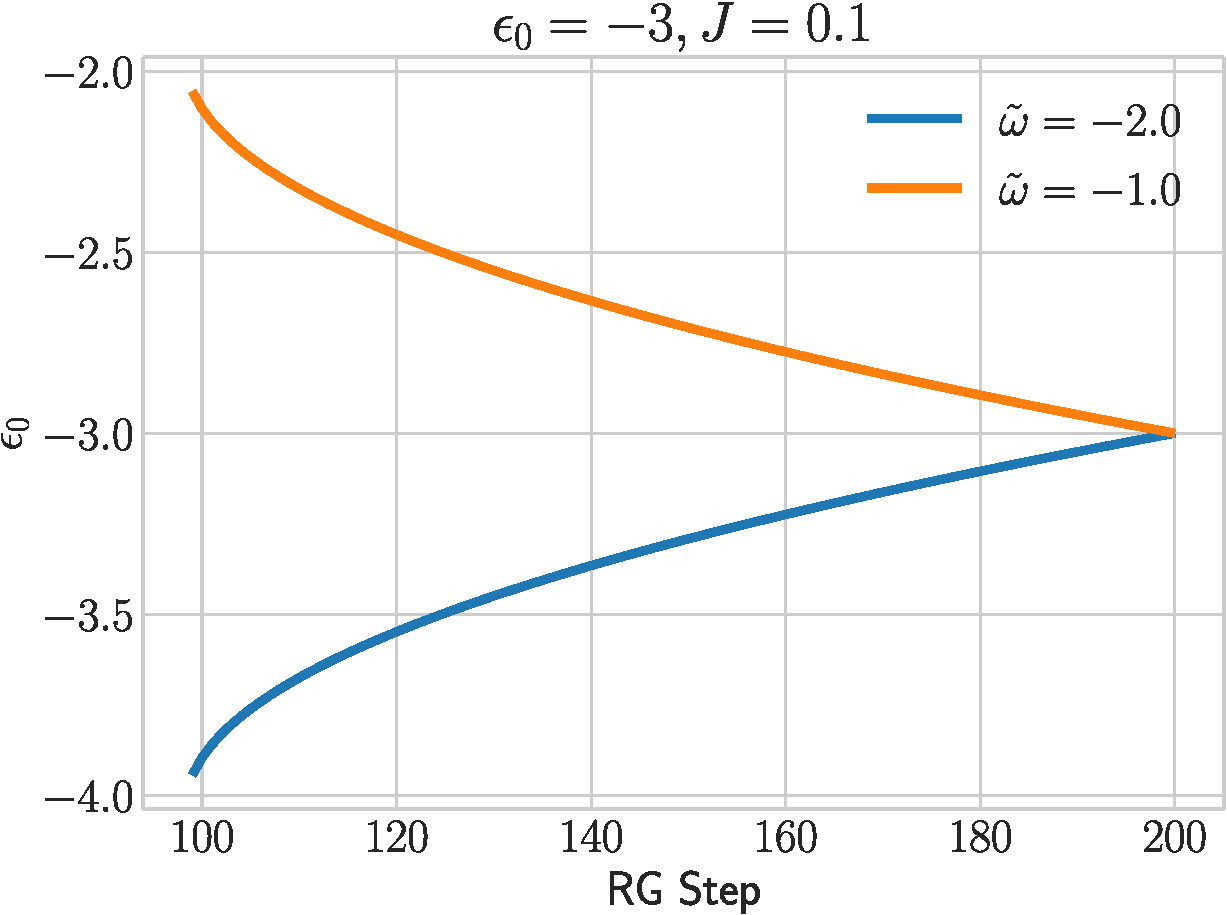
\includegraphics[width=0.45\textwidth]{../figures/notzero1.pdf}
	\hspace*{\fill}
	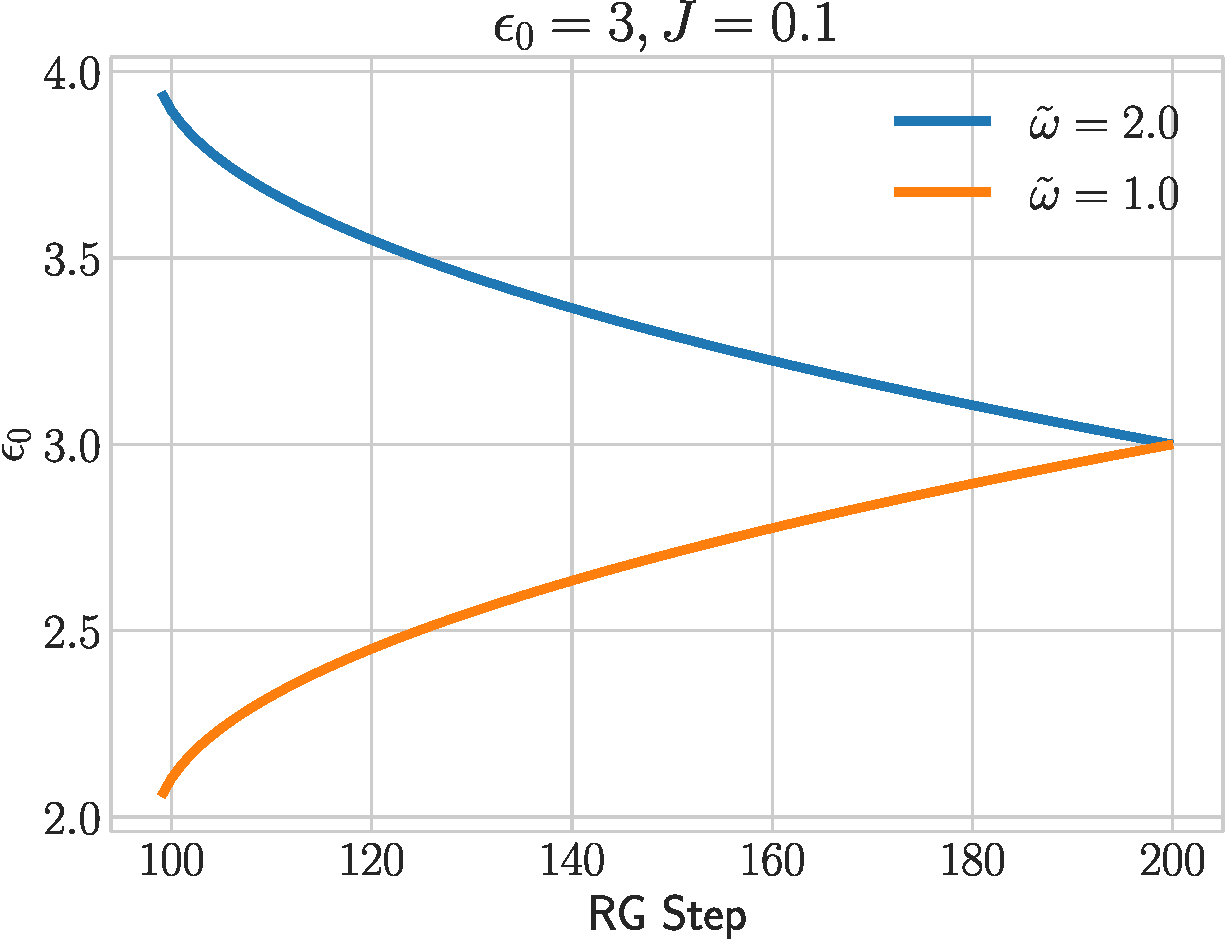
\includegraphics[width=0.45\textwidth]{../figures/notzero2.pdf}
	\captionof{figure}{Flows where \(\epsilon_0\) and \(\tilde\omega\) have same sign. The left and right panels show flows starting from negative and positive values respectively. The two plots in each panel correspond to different values of \(\tilde \omega\), one greater than the bare \(\epsilon_0\), the other less than that. The fixed point value is \(2\tilde\omega\).}
	\label{plot1}
\end{center}
\begin{center}
	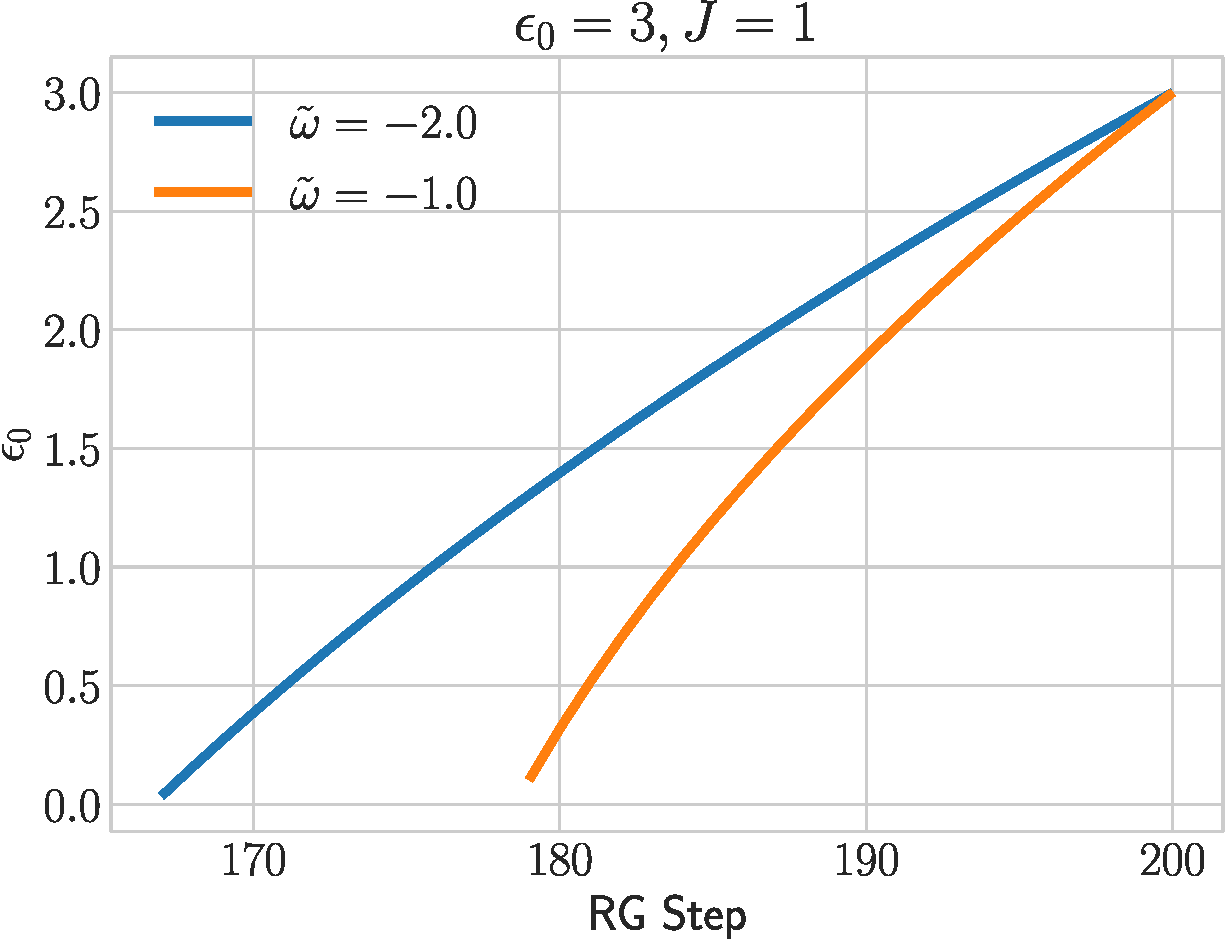
\includegraphics[width=0.45\textwidth]{../figures/zero2.pdf}
	\hspace*{\fill}
	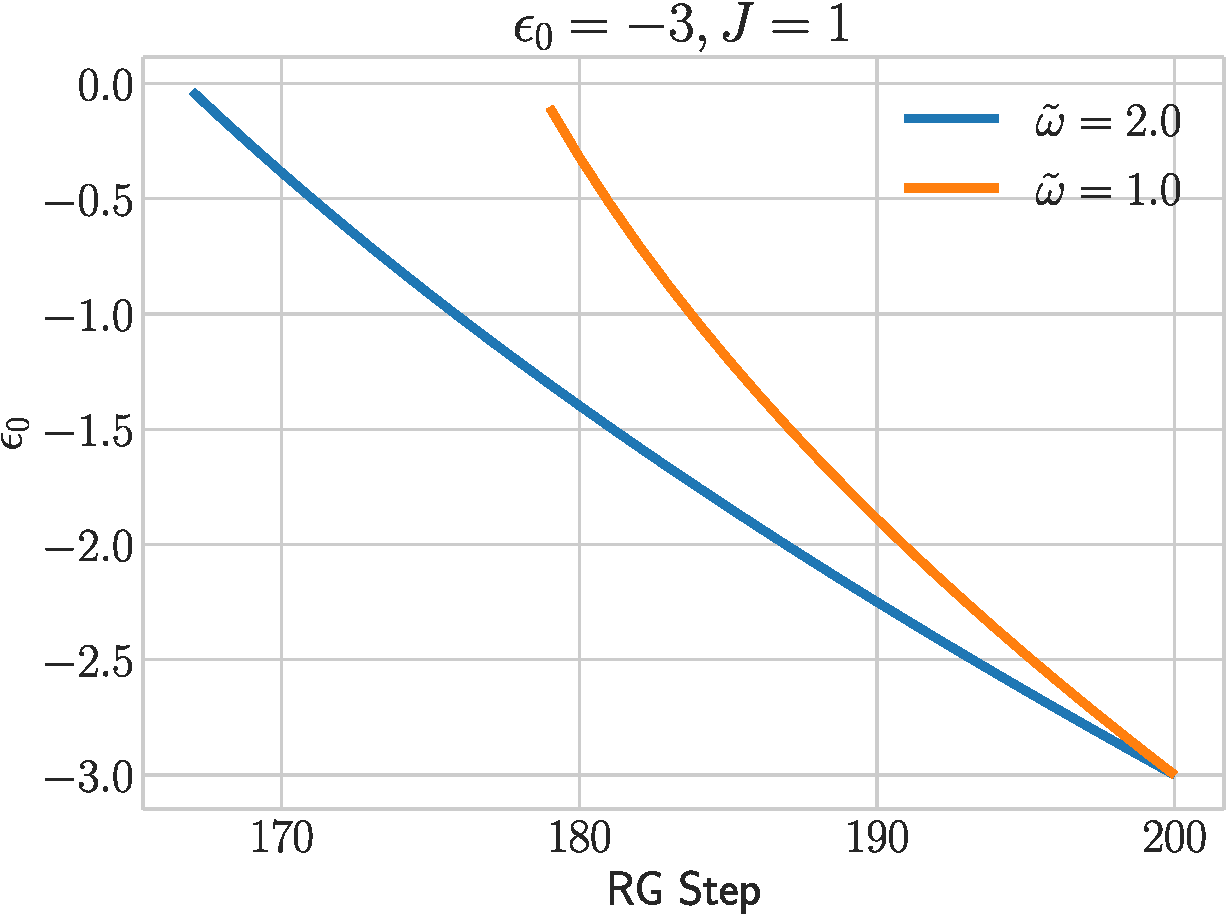
\includegraphics[width=0.45\textwidth]{../figures/zero1.pdf}
	\captionof{figure}{Flows where \(\epsilon_0\) and \(\tilde\omega\) have opposite sign. The left and right panels show flows starting from negative and positive values respectively. The two plots in each panel correspond to different values of \(\tilde \omega\), one greater than the bare \(\epsilon_0\), the other less than that. The fixed point value is 0.}
	\label{plot2}
\end{center}
\section{URG analysis of the single-channel Kondo model}
\label{kondourg}
The Kondo model URG analysis was originally carried out in ref.~\cite{am_thesis}. A specific version of the model is described by the Hamiltonian
\begin{equation}\begin{aligned}
	\mathcal{H} = \sum_{k\sigma}\epsilon_{k}\tau_{k\sigma} + \sum_{k,l} J^z S_d^z s^z_{kl} + \frac{1}{2}\sum_{k,l} J^t \left(S_d^+ s^-_{kl}  + S_d^- s^+_{kl}\right)
\end{aligned}\end{equation}
where \(s^z_{kl} = \frac{1}{2}\left(c^\dagger_{k\uparrow}c_{l \uparrow} - c^\dagger_{k\downarrow}c_{l \downarrow}\right)\), \(s^-_{kl} = c^\dagger_{k \downarrow}c_{l \uparrow}\) and \(s^+_{kl} = {s^-_{lk}}^\dagger\). Also, \(\tau = \hat n - \frac{1}{2}\). \(k,l\) sum over the momentum states. \(\vec S_d\) is the impurity spin operator.

The scheme is that we will disentangle an electron \(q\beta\) from the Hamiltonian, \(q\) being the momentum and \(\beta\) the spin. The diagonal part of the Hamiltonian under this scheme is
\begin{equation}\begin{aligned}
\label{kondodiag}
H^D_{q\beta} = \epsilon_q \tau_{q\beta} + J^z S_d^z s_{qq}^z
\end{aligned}\end{equation}
The off-diagonal parts at a particular RG step \(H^I_1\) and \(H^I_0\), that start from particle and hole states respectively, are
\begin{equation}\begin{aligned}
	H^I_1 = \sum_{|k|<\Lambda,q} J^z S_d^z s^z_{kq} + \frac{1}{2}\sum_{|k|<\Lambda,q} J^t \left(S_d^+ s^-_{kq} + S_d^- s^+_{kq}\right)\\
	H^I_0 = \sum_{|k|<\Lambda,q} J^z S_d^z s^z_{qk} + \frac{1}{2}\sum_{|k|<\Lambda,q} J^t \left(S_d^+ s^-_{qk}  + S_d^- s^+_{qk}\right)
\end{aligned}\end{equation}
\(H^I_1\) is the Hamiltonian term that scatters from the occupied configuration of \(q\), \(H^I_0\) is the same from the unoccupied configuration.
These are the terms that appear in the numerator.
\subsection{Particle sector}
The particle sector involves integrating out those states which are occupied (\(\hat n_{q\beta}=1\)). We will work at an energy  shell \(\epsilon_q = -D\). The renormalization is
\begin{equation}\begin{aligned}
	H^I_0 \frac{1}{\omega - H^D_{q\beta}} H^I_1
\end{aligned}\end{equation}

Both \(H^I_0\) and \(H^I_1\) have all three operators \(S_d^z, S_d^\pm\). We call \(S_d^z\) the spin-keep term and the others spin-flip terms. The entire product will thus have \(3\times 3 = 9\) terms. Not all terms however renormalize the Hamiltonian. Those terms that have identical operators on both sides can be ignored because \({S_d^z}^2 = \text{constant}\) and \({S^\pm}^2 = 0\). The other six terms will renormalize the Hamiltonian. This brings in one more simplification: all the six terms that \textit{will} renormalize the Hamiltonian have a spin flip operator on at least one side of the Greens function. This means that in the denominator of the Greens function, \(S_d^z\) and \(s^z_{qq}\) have to be anti-parallel in order to produce a non-zero result for that term. This means we can identically replace \(S_d^z s^z_{qq} = -\frac{1}{4}\). Also, in the particle sector, the Greens function always has \(c_{q\beta}\) in front of it, so \(\epsilon_q \tau_{q\beta} = D/2\). Substituting all this, we get
\begin{equation}\begin{aligned}
	\frac{1}{\omega - D/2 + J/4}\sum_{|k,k^\prime|<\Lambda,q}\left[\frac{1}{2}J^z J^t \left(S_d^z S_d^+ s^z_{qk^\prime}s^-_{kq} + S_d^z S_d^- s^z_{qk^\prime}s^+_{kq}\right) + \frac{1}{2}J^t J^z \left(S_d^+ S_d^z s^-_{qk^\prime}s^z_{kq} + S_d^- S_d^z s^+_{qk^\prime}s^z_{kq}\right)\right.\\
+\left.\frac{1}{4}{J^t}^2 \left(S_d^- S_d^+ s^+_{qk^\prime}s^-_{kq} + S_d^+ S_d^- s^-_{qk^\prime}s^+_{kq}\right)\right]
\end{aligned}\end{equation}
We now simplify the products and keep only terms diagonal in \(q\). For example: \(s^z_{qk^\prime}s^+_{kq} = \frac{1}{2}\hat n_{q \downarrow}s^+_{kk^\prime}\) and \(s^z_{qk^\prime}s^-_{kq} = -\frac{1}{2}\hat n_{q \uparrow}s^-_{kk^\prime}\). The renormalization becomes
\begin{equation}\begin{aligned}
	\frac{1}{\omega - D/2 + J/4}\sum_{|k,k^\prime|<\Lambda,q}\left[\frac{1}{4}J^z J^t \left(-\frac{1}{2}S_d^+ \hat n_{q}s^-_{kk^\prime} - \frac{1}{4}S_d^- \hat n_{q} s^z_{kk^\prime}\right) - \frac{1}{4}{J^t}^2 S_d^z\left(-\hat n_{q \uparrow}c^\dagger_{k \downarrow}c_{k^\prime \downarrow} + \hat n_{q \downarrow}c^\dagger_{k \uparrow}c_{k^\prime \uparrow}\right)\right]
\end{aligned}\end{equation}
We now replace \(\sum_q \hat n_{q\sigma} = n(D)\). The renormalization due to excitations coming from the particle sector is
\begin{equation}\begin{aligned}
	\Delta H_1 = -\frac{1}{2}\frac{n(D)}{\omega - D/2 + J/4}\sum_{|k,k^\prime|<\Lambda}\left[J^z J^t \frac{1}{2}\left(S_d^+ s^-_{kk^\prime} + S_d^- s^z_{kk^\prime}\right) + {J^t}^2 S_d^z s^z_{kk^\prime}\right]
\end{aligned}\end{equation}
The renormalization in the couplings coming from the particle sector is therefore,
\begin{equation}\begin{aligned}
	\label{kondo_part}
	\Delta J^z = -\frac{1}{2}\frac{{J^t}^2n(D)}{\omega - D/2 + J/4}, && \Delta J^t = -\frac{1}{2}\frac{J^z J^tn(D)}{\omega - D/2 + J/4}
\end{aligned}\end{equation}


\subsection{Hole sector}
The hole sector involves integrating out those states which are vacant (\(\hat n_{q\beta}=1\)). We will work at an energy  shell \(\epsilon_q = D\). The renormalization is
\begin{equation}\begin{aligned}
	H^I_1 \frac{1}{\omega - H^D_{q\beta}} H^I_0
\end{aligned}\end{equation}
The same considerations as those in the particle sector apply here, and the denominator becomes \(\omega - D/2 + J/4\), while the numerator is \(H^I_1 H^I_0\). Since this is just the Hermitian conjugate of the particle sector form, we do not need to calculate this separately, because the renormalization here will be \(\Delta H_0 = \Delta H_1^\dagger = \Delta H_1\).

\subsection{Scaling equations}
Since the renormalization in the hole sector is equal to that in the particle sector, the total renormalization is simply twice that in the particle sector (eqs.~\ref{kondo_part}):
\begin{equation}\begin{aligned}
	\Delta J^z = -\frac{{J^t}^2n(D)}{\omega - D/2 + J/4}, && \Delta J^t = -\frac{J^z J^tn(D)}{\omega - D/2 + J/4}
\end{aligned}\end{equation}
If we set \(J_z = J_t = J\), we have an SU(2)-symmetric Kondo model \(J \vec{S_d}\cdot\vec{s}\).
\begin{equation}\begin{aligned}
	\label{kondosym}
	\Delta J = - \frac{J^2 n(D)}{\omega - D/2 + \frac{1}{4}J}
\end{aligned}\end{equation}
To recover the one-loop form, we can replace \(\omega\) with the bare value \(-D/2\) and ignore the \(J\) in the denominator (small \(J\)).
\begin{equation}\begin{aligned}
	\Delta J \approx \frac{J^2 n(D)}{D}
\end{aligned}\end{equation}
\subsection{Numerical Solutions}
The symmetric scaling equation \ref{kondosym} was solved numerically with the choice \(\omega = -\frac{\epsilon_q}{2}\), for both positive and negative bare values of \(J\). For sufficiently low values of \(\omega\), the Kondo coupling \(J\) flows to the strong-coupling limit. This limit, as obtained from the URG, is of course finite. This can be reconciled with the NRG result \(J^* = \infty\) by noting the fact that increasing the bare bandwidth \(D\) does increase the value of URG \(J^*\), such that in the thermodynamic limit \(D \to \infty\), URG should give \(J^* \to \infty\). This is shown in fig.~\ref{JvsD-kondo}

\begin{figure}[!htpb]
	\centering
	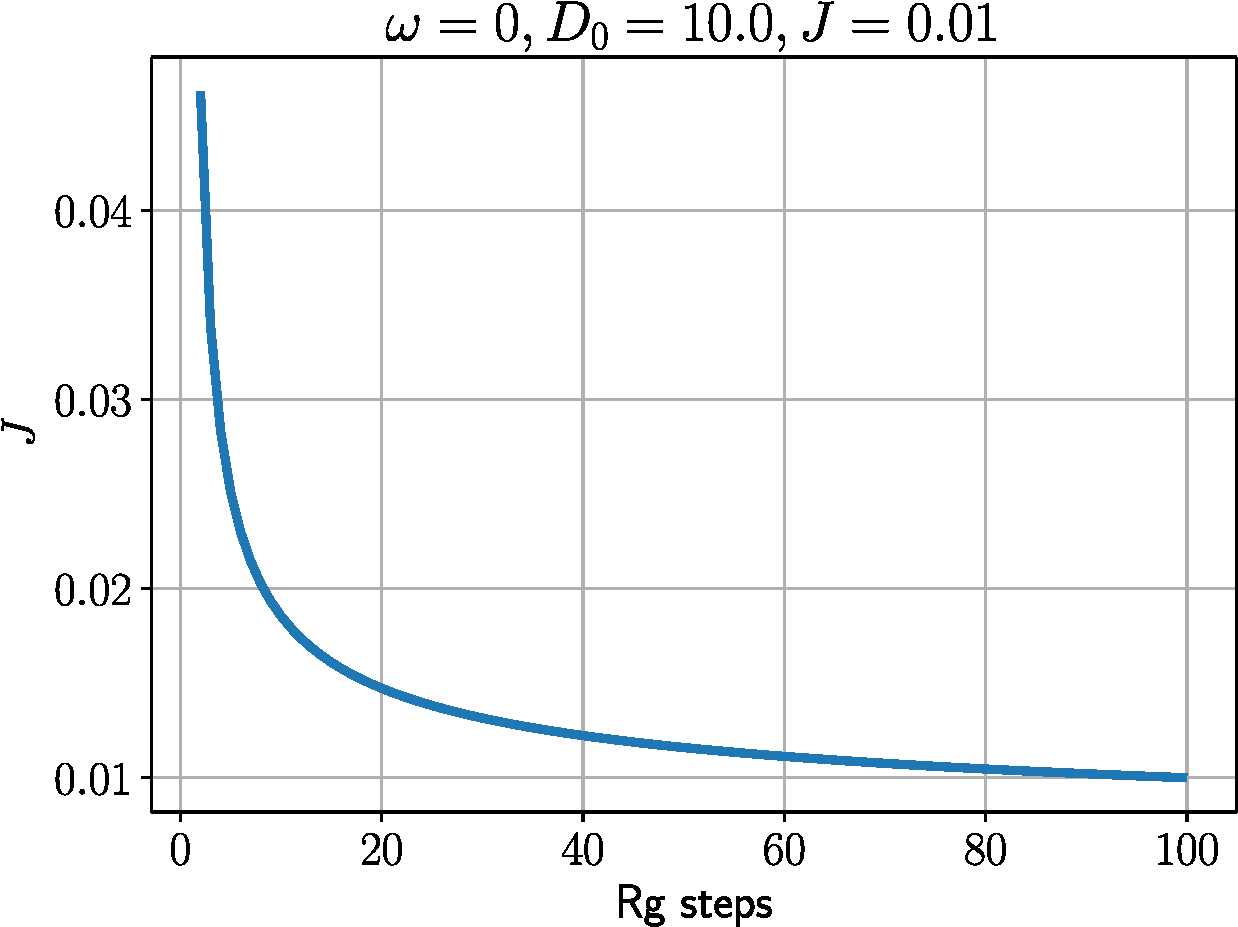
\includegraphics[width=0.45\textwidth]{../figures/relJ.pdf}
	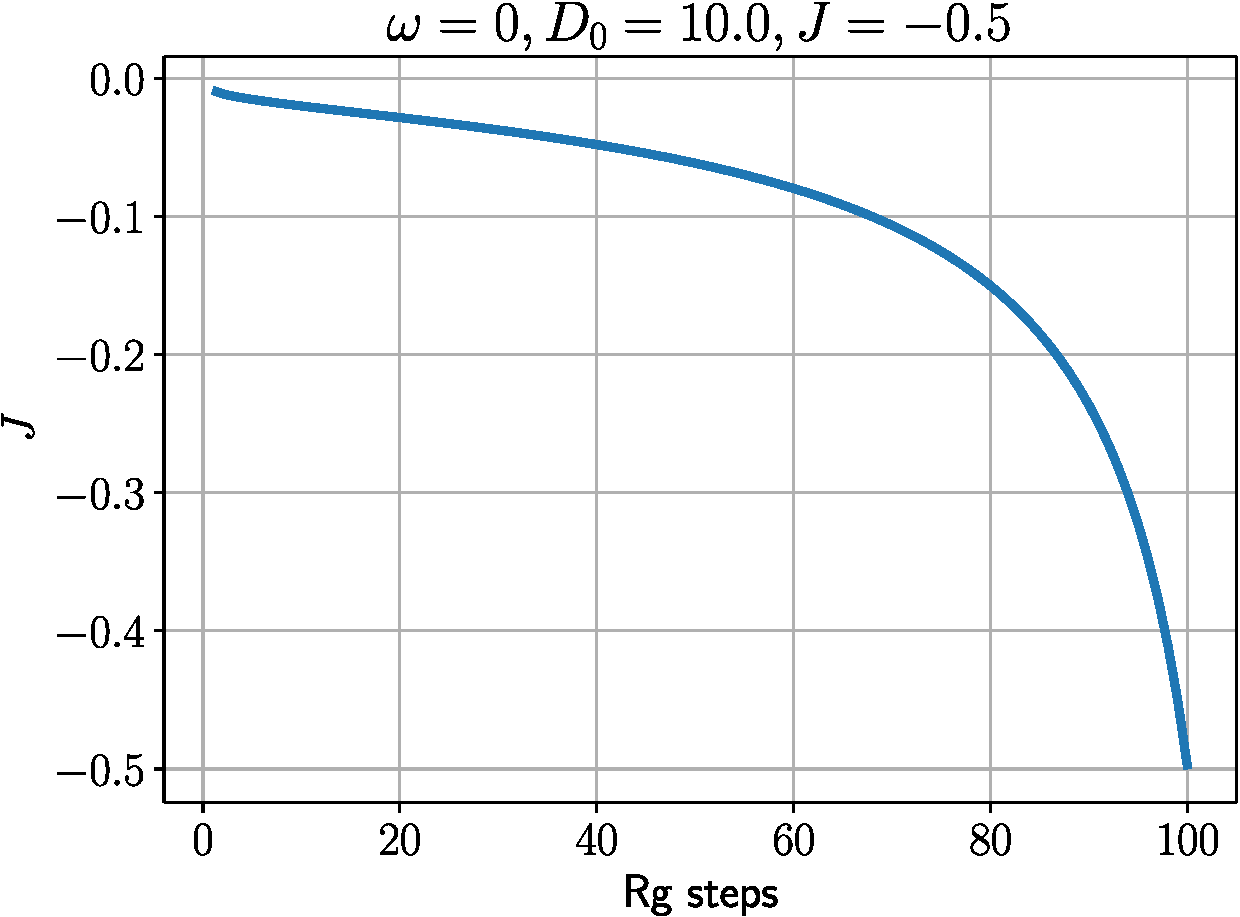
\includegraphics[width=0.45\textwidth]{../figures/rel2J.pdf}
	\caption{Flow of \(J\) towards the strong-coupling fixed point (right) and the weak coupling saddle-point (left).  The x-axis indicates the index of the energy shell being decoupled. The largest value (UV) is the first step, and we go towards the left (IR).}
\end{figure}

\begin{figure}[!htpb]
	\centering
	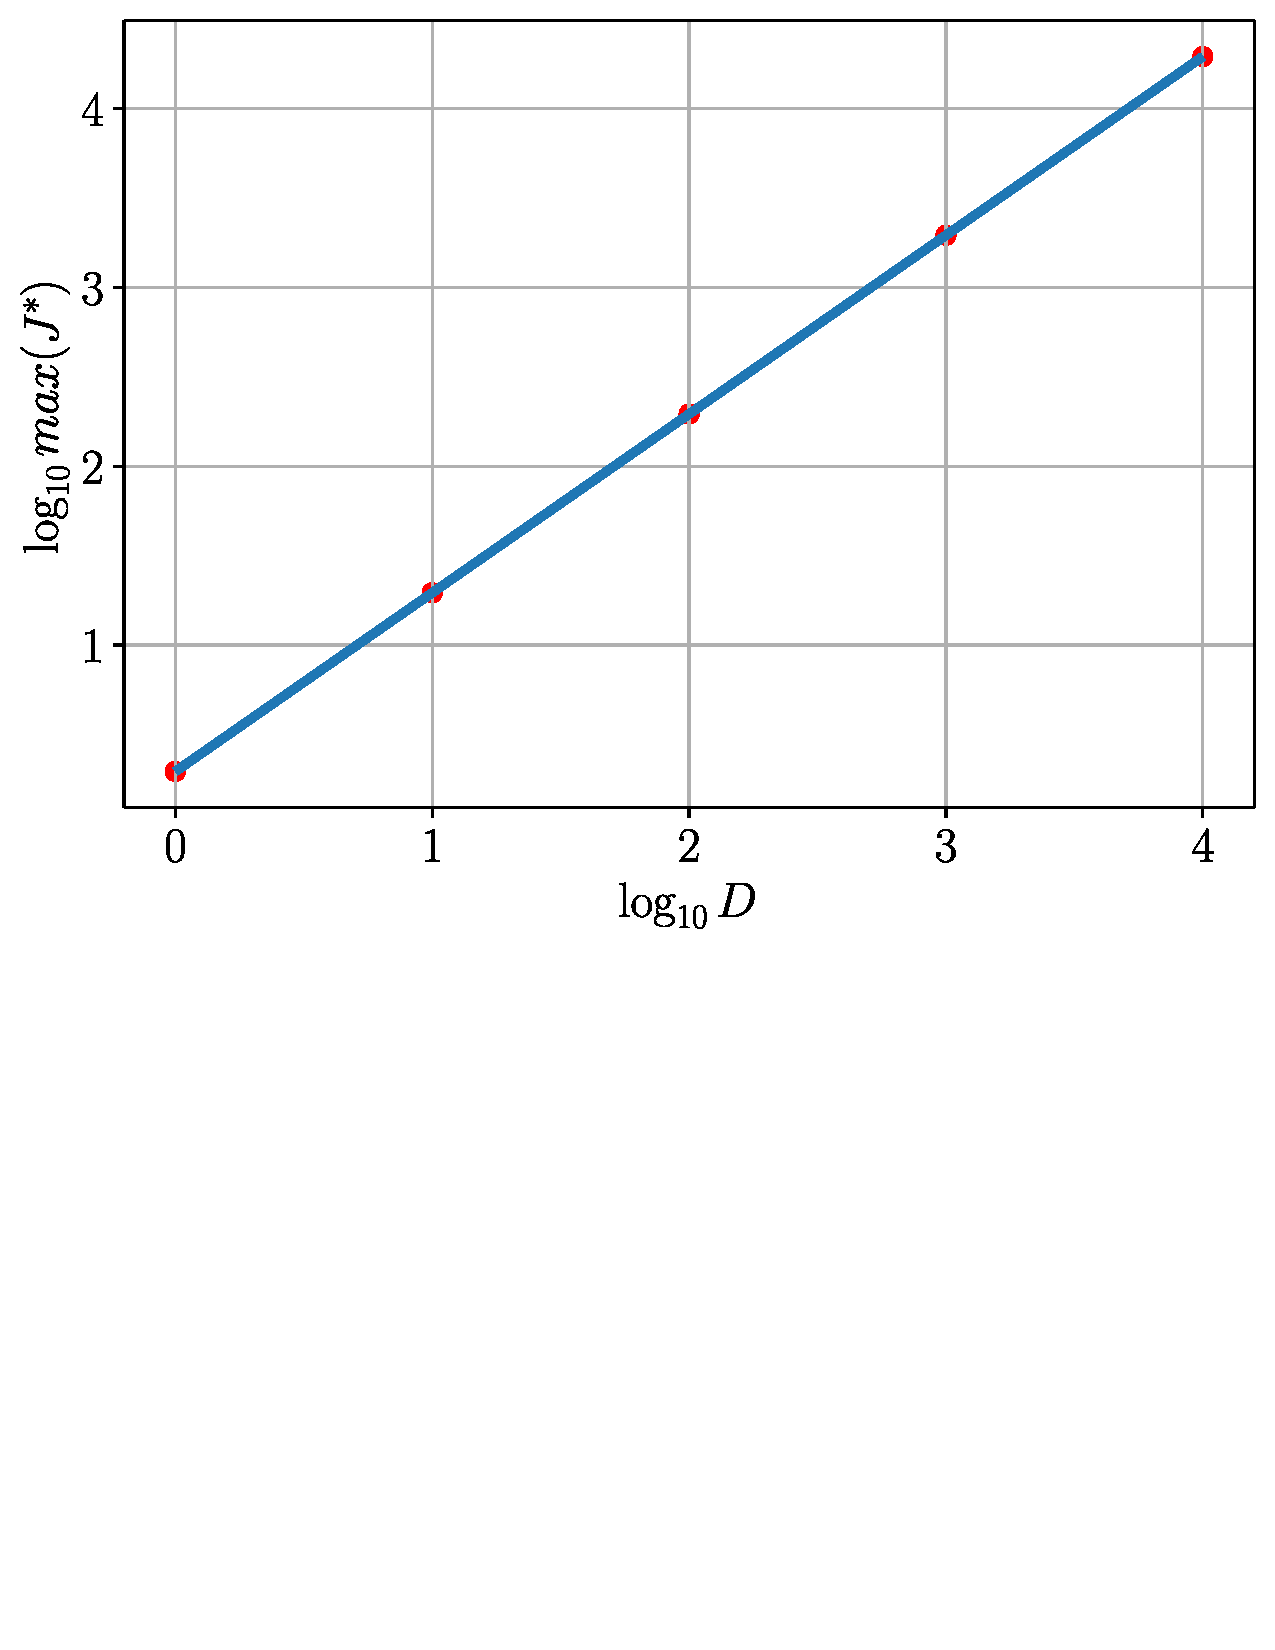
\includegraphics[scale=0.4]{../figures/JvsD_kondo.pdf}
	\caption{Variation of the fixed point value \(J^*\) against the bare bandwidth, in log scale.}
	\label{JvsD-kondo}
\end{figure}

\section{URG analysis of the multi-channel Kondo model}

\subsection{Introduction}
The multi-channel Kondo model is described by the Hamiltonian
\begin{equation}\begin{aligned}
	H = \sum_{k,\alpha,\gamma}\epsilon_{k}^\gamma \hat n^\gamma_{k\alpha} + J\sum_{kk^\prime,\gamma} \vec{S_d}\cdot\vec{s}_{\alpha\alpha^\prime}{c^\gamma_{k\alpha}}^\dagger c^\gamma_{k^\prime\alpha^\prime}~.
\end{aligned}\end{equation}
It is mostly identical to the single-channel Kondo model: \(k,k^\prime\) sum over the momentum states, \(\alpha,\alpha^\prime\) sum over the spin indices and \(\gamma\) sums over the various channels. \(\vec S_d, \vec s\) are the impurity and conduction bath spin vectors. The renormalization at step \(j\) is given by
\begin{equation}\begin{aligned}
	\Delta H_j = \left(c^\dagger T \frac{1}{\hat \omega - H_D}T^\dagger c + T^\dagger c \frac{1}{\hat \omega - H_D}c^\dagger T\right), && c^\dagger T = J \sum_{k < \Lambda_j, \alpha}\vec{S_d}\cdot\vec{s}_{\beta \alpha}c^\dagger_{q\beta}c_{k\alpha}, &H_D = \epsilon_q \tau_{q\beta} + J S_d^z s_q^z
\end{aligned}\end{equation}
Usually we treat the \(\hat \omega\) as number(s) and study the renormalization in the couplings as functions of the quantum fluctuation scales. Each value of the fluctuation scale defines an eigendirection of \(\hat \omega\). We have then essentially traded off the complexity in the non-commutation of the diagonal and off-diagonal terms for all the directions in the manifold of \(\hat \omega\).

Here we will do something different. We will redefine the \(\hat \omega\) by pulling out the off-diagonal term from it: \(\hat \omega \to \hat \omega - H_X\), and then study the renormalization at various orders by expanding the denominator in powers of \(H_X\). Such a redefinition essentially amounts to a rotation of the eigendirections of \(\hat \omega\). This is done in order to extract some information out of \(\hat \omega\), specifically the dependence of the RG equations on the channel number \(K = \sum_\gamma\). This dependence is in principle present even if we do not do such a redefinition and expansion, in the various directions and values of \(\omega\), because those values encode the non-perturbative information regarding scattering at all loops. However, it is difficult to read off this information directly. This step of redefinition followed by expansion is being done with the sole aim of exposing such information. 

The expansion we are talking about is
\begin{equation}\begin{aligned}
	\eta = \frac{1}{\hat \omega - H_D}T^\dagger c = \frac{1}{\omega^\prime - H_D - H_X}T^\dagger c \simeq \frac{1}{\omega^\prime - H_D}T^\dagger c + \frac{1}{\omega^\prime - H_D}H_X \frac{1}{\omega^\prime - H_D} T^\dagger c
\end{aligned}\end{equation}
where \(H_X = J \sum_{k,k^\prime < \Lambda_j, \alpha,\alpha^\prime}\vec{S_d}\cdot\vec{s}_{\alpha \alpha^\prime}c^\dagger_{k\alpha}c_{k^\prime\alpha^\prime}\) is scattering between the entangled electrons.
With this change, the second and third order renormalizations will take the form
\begin{equation}\begin{aligned}
	\Delta H^{(2)}_j = c^\dagger T \frac{1}{\omega^\prime - H_D}T^\dagger c + T^\dagger c \frac{1}{\omega - H_D}c^\dagger T
\end{aligned}\end{equation}
\begin{equation}\begin{aligned}
	\Delta H^{(3)}_j = c^\dagger T \frac{1}{\omega^\prime - H_D} H_X \frac{1}{\omega^\prime - H_D} T^\dagger c + T^\dagger c \frac{1}{\omega - H_D} H_X \frac{1}{\omega - H_D} c^\dagger T
\end{aligned}\end{equation}
We will use the identity
\begin{equation}\begin{aligned}
	\label{identity_SSS}
	S_d^a S_d^z S_d^b = \left(\frac{1}{4}\delta^{az} + \frac{i}{2}\sum_c \epsilon^{azc}S_d^c\right)S_d^b = \left(\frac{1}{4}\delta^{az}S_d^b + \frac{i}{8} \epsilon^{azb}  - \frac{1}{4}\sum_{c_1,c} \epsilon^{azc_1} \epsilon^{c_1 b c} S_d^c\right) = \frac{1}{4}\left(\delta^{az}S_d^b - \delta^{ab}S_d^z + \delta^{bz}S_d^a\right)
\end{aligned}\end{equation}

\subsection{Leading order renormalization}
\begin{equation}\begin{aligned}
	\Delta H^{(2)}_j = \underbrace{c^\dagger T \frac{1}{\omega^\prime - H_D}T^\dagger c}_\text{first term}~+~\underbrace{T^\dagger c \frac{1}{\omega - H_D}c^\dagger T}_\text{second term}
\end{aligned}\end{equation}
This renormalization is identical to that in the single channel. There is no additional physics due to the presence of multiple channels at this order.
\begin{equation}\begin{aligned}
	\Delta J^{(2)} = -\frac{J^2 n(D)}{\omega - D/2 + J/4}
\end{aligned}\end{equation}
For \(\omega < D/2\), we get the flow towards the strong-coupling fixed point. That is, there appears a stable fixed point at \(J^* = 4|\omega - D/2|\) for all bare \(J > 0\). We also get a decay towards the local moment fixed point \(J^* = 0\) for \(J < 0\). For \(\omega = -D/2\) and \(J \ll D\), we get the one-loop PMS form. 
\begin{equation}\begin{aligned}
	\Delta J^{(2)} = \frac{J^2 n(D)}{D - J/4} \simeq \frac{J^2 n(D)}{D}
\end{aligned}\end{equation}
\subsection{Next-to-leading order renormalization}
\begin{equation}\begin{aligned}
	\Delta H^{(3)}_j = \underbrace{c^\dagger T \frac{1}{\omega^\prime - H_D} H_X \frac{1}{\omega^\prime - H_D} T^\dagger c}_\text{first term} ~+~ \underbrace{T^\dagger c \frac{1}{\omega - H_D} H_X \frac{1}{\omega - H_D} c^\dagger T}_\text{second term}
\end{aligned}\end{equation}
A general term of this summation has three sets of spin operators coming from \(c^\dagger T, H_X\) and \(T^\dagger c\). If we had expressed the spin operators in terms of \(S^z, S^\pm\), most of the terms would have atleast one \(S^+\) or \(S^-\), and by the same argument as in the single-channel case, the denominator will have anti-parallel spins and the Ising term will be negative, leading to the form: \(\omega - D/2 - \epsilon_k/2 + J/4\). \(\epsilon_k\) is the energy of the other electron that will be summed over. The only term that does not have even one \(S^\pm\) is the one with three \(S^z\). We can show that this term will also have the same denominator. An instance of this term (in shorthand) is
\begin{equation}\begin{aligned}
	S_d^z c^\dagger_{q \uparrow} \frac{1}{\omega - D/2 -\epsilon_k/2 + J/2 S_d^z} S_d^z \frac{1}{\omega - D/2 -\epsilon_k/2 + J/2 S_d^z} S_d^z c_{q \uparrow}\\
\end{aligned}\end{equation}
This can be split into up and down configurations of the impurity spin using the decomposition \(S_d^z = \frac{1}{2}\left(\frac{1}{2} + S_d^z\right) - \frac{1}{2}\left(\frac{1}{2} - S_d^z \right) \). These configurations will have different quantum fluctuation scales \(\omega, \omega^\prime\):
\begin{equation}\begin{aligned}
	\frac{1}{2}S_d^z c^\dagger_{q \uparrow}\left[\frac{\left(\frac{1}{2} + S_d^z\right)}{\left(\omega - D/2 -\epsilon_k/2 + J/4\right)^2} - \frac{\left(\frac{1}{2} - S_d^z\right)}{\left(\omega^\prime - D/2 -\epsilon_k/2 - J/4\right)^2}\right]S_d^z c_{q \uparrow}
\end{aligned}\end{equation}
If we now use poor man's scaling values to relate the two \(\omega\)s, we get \(\omega^\prime - \omega = J/2\). Substituting this will make both the denominators identical: \(\omega - D/2 -\epsilon_k/2 + J/4\). This means that the denominator for all non-zero terms that renormalize the Hamiltonian is \(\omega - D/2 - \epsilon_k/2 + J/4\).

\subsubsection{Calculation of first term}
\begin{equation}\begin{aligned}
	c^\dagger T \frac{1}{\omega^\prime - H_D} H_X \frac{1}{\omega^\prime - H_D} T^\dagger c = J^3\sum_{q, k, k_1,k_2,\atop{\beta, \alpha, \alpha_1,\alpha_2,\atop{l_1,l_2,a,b,c}}} \frac{c^\dagger_{q\beta,l_1} c_{k\alpha,l_1} S_d^a s^a_{\beta \alpha} S_d^b s^b_{\alpha_1 \alpha_2} c^\dagger_{k_1\alpha_1,l_2}c_{k_2 \alpha_2,l_2} c^\dagger_{k\alpha, l_1} c_{q\beta, l_1} S_d^c s^c_{\alpha \beta}}{\left(\omega - D/2 -\epsilon_k/2 + J/4\right)^2}
\end{aligned}\end{equation}
\(q\) sums over the momenta being decoupled. \(k, k_1,k_2\) sum over the momenta not being decoupled. \(\beta, \alpha, \alpha_1,\alpha_2\) sum over the spin indices. \(l_1,l_2\) sum over the channels. We will start simplifying this equation by summing over \(q\). \(c^\dagger_{q\beta}\) and \(c_{q\beta}\) can be easily combined to form \(\hat n_{q\beta}\), because they anti-commute with the other momenta. The sum gives \(\sum_q \hat n_{q\beta l_1} = n(D) \). This gives
\begin{equation}\begin{aligned}
	c^\dagger T \frac{1}{\omega^\prime - H_D} H_X \frac{1}{\omega^\prime - H_D} T^\dagger c = J^3 n(D)\sum_{k, k_1,k_2,\atop{\beta, \alpha, \alpha_1,\alpha_2,\atop{l_1,l_2,a,b,c}}} \frac{c_{k\alpha,l_1} S_d^a s^a_{\beta \alpha} S_d^b s^b_{\alpha_1 \alpha_2} c^\dagger_{k_1\alpha_1,l_2}c_{k_2 \alpha_2,l_2} c^\dagger_{k\alpha, l_1} S_d^c s^c_{\alpha \beta}}{\left(\omega - D/2 -\epsilon_k/2 + J/4\right)^2}
\end{aligned}\end{equation}
The operators \(c^\dagger_{k\alpha}\) and its conjugate can be brought together without any change of sign because there will be an even number of flips. The sum over \(k\) gives
\begin{equation}\begin{aligned}
	\sum_k \frac{1 - \hat n_{k\alpha l_1}}{\left(\omega - D/2 -\epsilon_k/2 + J/4\right)^2} =  \rho\int \frac{d\epsilon\left[1 - \hat n(\epsilon)_{\alpha l_1}\right] }{\left(\omega - D/2 -\epsilon/2 + J/4\right)^2} = \rho\int_0^{D-2\left( \omega + J/4 \right) } \frac{d\epsilon}{\left(\omega - D/2 -\epsilon/2 + J/4\right)^2}
\end{aligned}\end{equation}
The integration goes over positive energies only because of the \(1 - \hat n\) operator; the upper limit of the integration is chosen so as to make the denominator double, because this preserves the symmetry of the denominator and this is what happens in poor man's scaling. Performing the integration gives
\begin{equation}\begin{aligned}
	\sum_k \frac{1 - \hat n_{k\alpha l_1}}{\left(\omega - D/2 -\epsilon_k/2 + J/4\right)^2} = -\frac{1}{2}\frac{\rho}{\omega - D/2 + J/4}
\end{aligned}\end{equation}
The sum over the channel index \(l_1\) produces a factor of \(K\). \(K = \sum_{l_1}\) is the total number of conduction bath channels. The entire expression is now
\begin{equation}\begin{aligned}
	\label{first_term}
	c^\dagger T \frac{1}{\omega^\prime - H_D} H_X \frac{1}{\omega^\prime - H_D} T^\dagger c = -\frac{1}{2}\frac{J^3 n(D) \rho K}{\omega - D/2 + J/4}\sum_{\beta, \alpha, \alpha_1,\alpha_2,\atop{a,b,c}} S_d^a s^a_{\beta \alpha} S_d^b s^b_{\alpha_1 \alpha_2} S_d^c s^c_{\alpha \beta} \sum_{k_1,k_2,l_2} c^\dagger_{k_1\alpha_1,l_2}c_{k_2 \alpha_2,l_2}
\end{aligned}\end{equation}
We now need to simplify the spin products. The sum over \(\alpha,\beta\) can be carried out immediately: \(\sum_{\alpha,\beta} s^a_{\beta \alpha} s^c_{\alpha \beta} = \text{Trace}\left(s^a s^c\right) = \frac{1}{2}\delta^{ac}\). Substituting this gives
\begin{equation}\begin{aligned}
	c^\dagger T \frac{1}{\omega^\prime - H_D} H_X \frac{1}{\omega^\prime - H_D} T^\dagger c = -\frac{1}{2}\frac{J^3 n(D) \rho K}{\omega - D/2 + J/4}\frac{1}{2}\sum_{\alpha_1,\alpha_2,a,b} S_d^a S_d^b S_d^a \sum_{k_1,k_2,l_2} c^\dagger_{k_1\alpha_1,l_2}c_{k_2 \alpha_2,l_2}s^b_{\alpha_1 \alpha_2} 
\end{aligned}\end{equation}
The spin product can now be carried out:
\begin{equation}\begin{aligned}
	\sum_a S_d^a S_d^b S_d^a = \sum_a S_d^a\left[\frac{1}{4}\delta^{ab} + \frac{i}{2}\sum_c \epsilon^{bac}S_d^c\right] = \frac{1}{4}S_d^b - \frac{1}{4}\sum_{ace}\epsilon^{bac}\epsilon^{ace}S_d^e = \frac{1}{4}S_d^b - \frac{1}{4}S_d^b \sum_{ac}\epsilon^{bac}\epsilon^{acb} \\
	= -\frac{1}{4}S_d^b
\end{aligned}\end{equation}
The renormalization becomes
\begin{equation}\begin{aligned}
	\Delta H_1 = c^\dagger T \frac{1}{\omega^\prime - H_D} H_X \frac{1}{\omega^\prime - H_D} T^\dagger c = -\frac{1}{2}\frac{J^3 n(D) \rho K}{\omega - D/2 + J/4}\frac{1}{2}\left( -\frac{1}{4} \right) \sum_{k_1,k_2,\alpha_1,\alpha_2,b} S_d^b s^b_{\alpha_1 \alpha_2} c^\dagger_{k_1\alpha_1,l_2}c_{k_2 \alpha_2,l_2}\\
=\frac{1}{16}\frac{J^3 n(D) \rho K}{\omega - D/2 + J/4} \sum_{k_1,k_2,\alpha_1,\alpha_2} \vec{S_d}\cdot\vec{s}_{\alpha_1 \alpha_2} c^\dagger_{k_1\alpha_1,l_2}c_{k_2 \alpha_2,l_2}
\end{aligned}\end{equation}

\subsubsection{Calculation of second term}
Like the single-channel case, the renormalization coming from the hole excitations is exactly the Hermitian conjugate of that in the particle sector. And since the renormalization \(\Delta H_1\) is Hermitian, we have \(\Delta H_0 = \Delta H_1\)

\subsection{Total renormalization \(\Delta H^{(3)}\)}
The total renormalization is twice that in the particle sector.
\begin{equation}\begin{aligned}
	\Delta H^{(3)} = \frac{1}{8}\frac{J^3 n(D) \rho K}{\omega - D/2 + J/4} \sum_{k_1,k_2,\alpha_1,\alpha_2} \vec{S_d}\cdot\vec{s}_{\alpha_1 \alpha_2} c^\dagger_{k_1\alpha_1,l_2}c_{k_2 \alpha_2,l_2}
\end{aligned}\end{equation}
Combining with \(\Delta H^{(2)}\) and replacing \(n(D) = \rho |\delta D|\), we get
\begin{equation}\begin{aligned}
	\frac{\Delta J}{|\Delta D|} = -\frac{J^2 \rho}{\omega - D/2 + J/4} + \frac{1}{8}\frac{J^3 \rho^2 K}{\omega - D/2 + J/4} = -\frac{J^2 \rho}{\omega - D/2 + J/4}\left[1 - \frac{1}{8}J\rho K\right] 
\end{aligned}\end{equation}
We choose \(\omega = -D/2\) to get a clearer idea of what the equations say. 
\begin{equation}\begin{aligned}
	\label{mchannel}
	\frac{\Delta J}{|\Delta D|} = \frac{J^2 \rho}{D - J/4}\left[1 - \frac{1}{8}J\rho K\right] 
\end{aligned}\end{equation}
Quantities with zero in the subscript will denote their values in the bare Hamiltonian. Using \(\delta D = -|\delta D|\), we can write the continuum form of the equation:
\begin{equation}\begin{aligned}
	\frac{\:\mathrm{d}J}{\:\mathrm{d}D} = \frac{J^2 \rho}{D - J/4}\left(\frac{1}{8}J\rho K - 1\right)
\end{aligned}\end{equation}

For \(D \gg J\), we can ignore the \(J\) in the denominator, and the equation reduces to the one-loop poor man's scaling form
\begin{equation}\begin{aligned}
	\label{pms_mchannel}
	\frac{\:\mathrm{d}J}{\:\mathrm{d}D} \simeq  \frac{J^2 \rho}{D}\left(\frac{1}{8}J\rho K - 1\right)
\end{aligned}\end{equation}
This equation has a stable fixed point at \(J^* = \frac{8}{\rho K}\).

\begin{figure}[htpb]
	\centering
	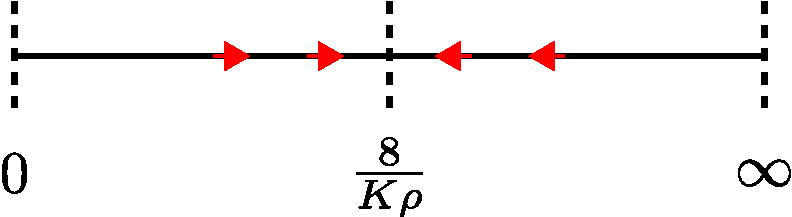
\includegraphics[width=0.4\textwidth]{rg_flow_pms.pdf}
	\caption{Attractive finite \(J\) fixed point of poor man scaling RG equation}
\end{figure}
For \(D\) not so large, the denominator also comes into play, and eq.\ref{mchannel} holds. We get the possibility of two fixed points - one from the numerator and the other from the numerator.
\begin{figure}[htpb]
	\centering
	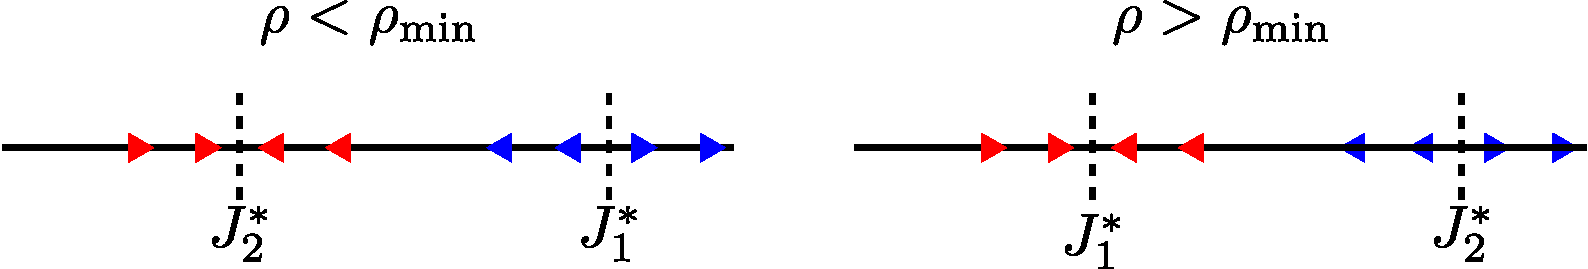
\includegraphics[width=0.7\textwidth]{./rg_flow.pdf}
	\caption{}
	\label{rg_flow_general}
\end{figure}

The numerator and denominator fixed points, \(J_1^*\) and \(J_2^*\) respectively, are given by
\begin{equation}\begin{aligned}
	J_1^* = \frac{8}{K \rho}, && D^* = \frac{J_2^*}{4}
\end{aligned}\end{equation}
For a given \(K\), the position of \(J_1^*\) will be governed by \(\rho\). In general, for each bare bandwidth \(D_0\), there exists a minimal \(\rho\), $\rho_\text{min}(D_0)$, above which the the lower fixed point is the one from the numerator. That is, for \(\rho > \rho_\text{min}\), if we start scaling from small \(J_0\), it grows until it hits \(J_1^*\) which acts as the attractive fixed point, and \(J_2^*\) lies at a higher value and acts as the repulsive fixed point. For \(\rho < \rho_\text{min}\), \(J\) will grow and hit \(J_2^*\) instead, and \(J_1^* > J_2^*\) now becomes the repulsive fixed point.
\begin{equation}\begin{aligned}
	\rho_\text{min} = \text{minimum }\left\{\rho, \text{ such that } \frac{8}{K \rho} < 4 D^*(\rho)\right\}
\end{aligned}\end{equation}
This behaviour is shown schematically in fig.~\ref{rg_flow_general}. 
In fig.~\ref{rhomin_vs_D}, we plot \(\rho_\text{min}\) against the bare bandwidth. For large \(D_0\), it essentially shrinks to zero, and the numerator becomes the first fixed point for essentially all \(\rho\).
\begin{figure}[htpb]
	\centering
	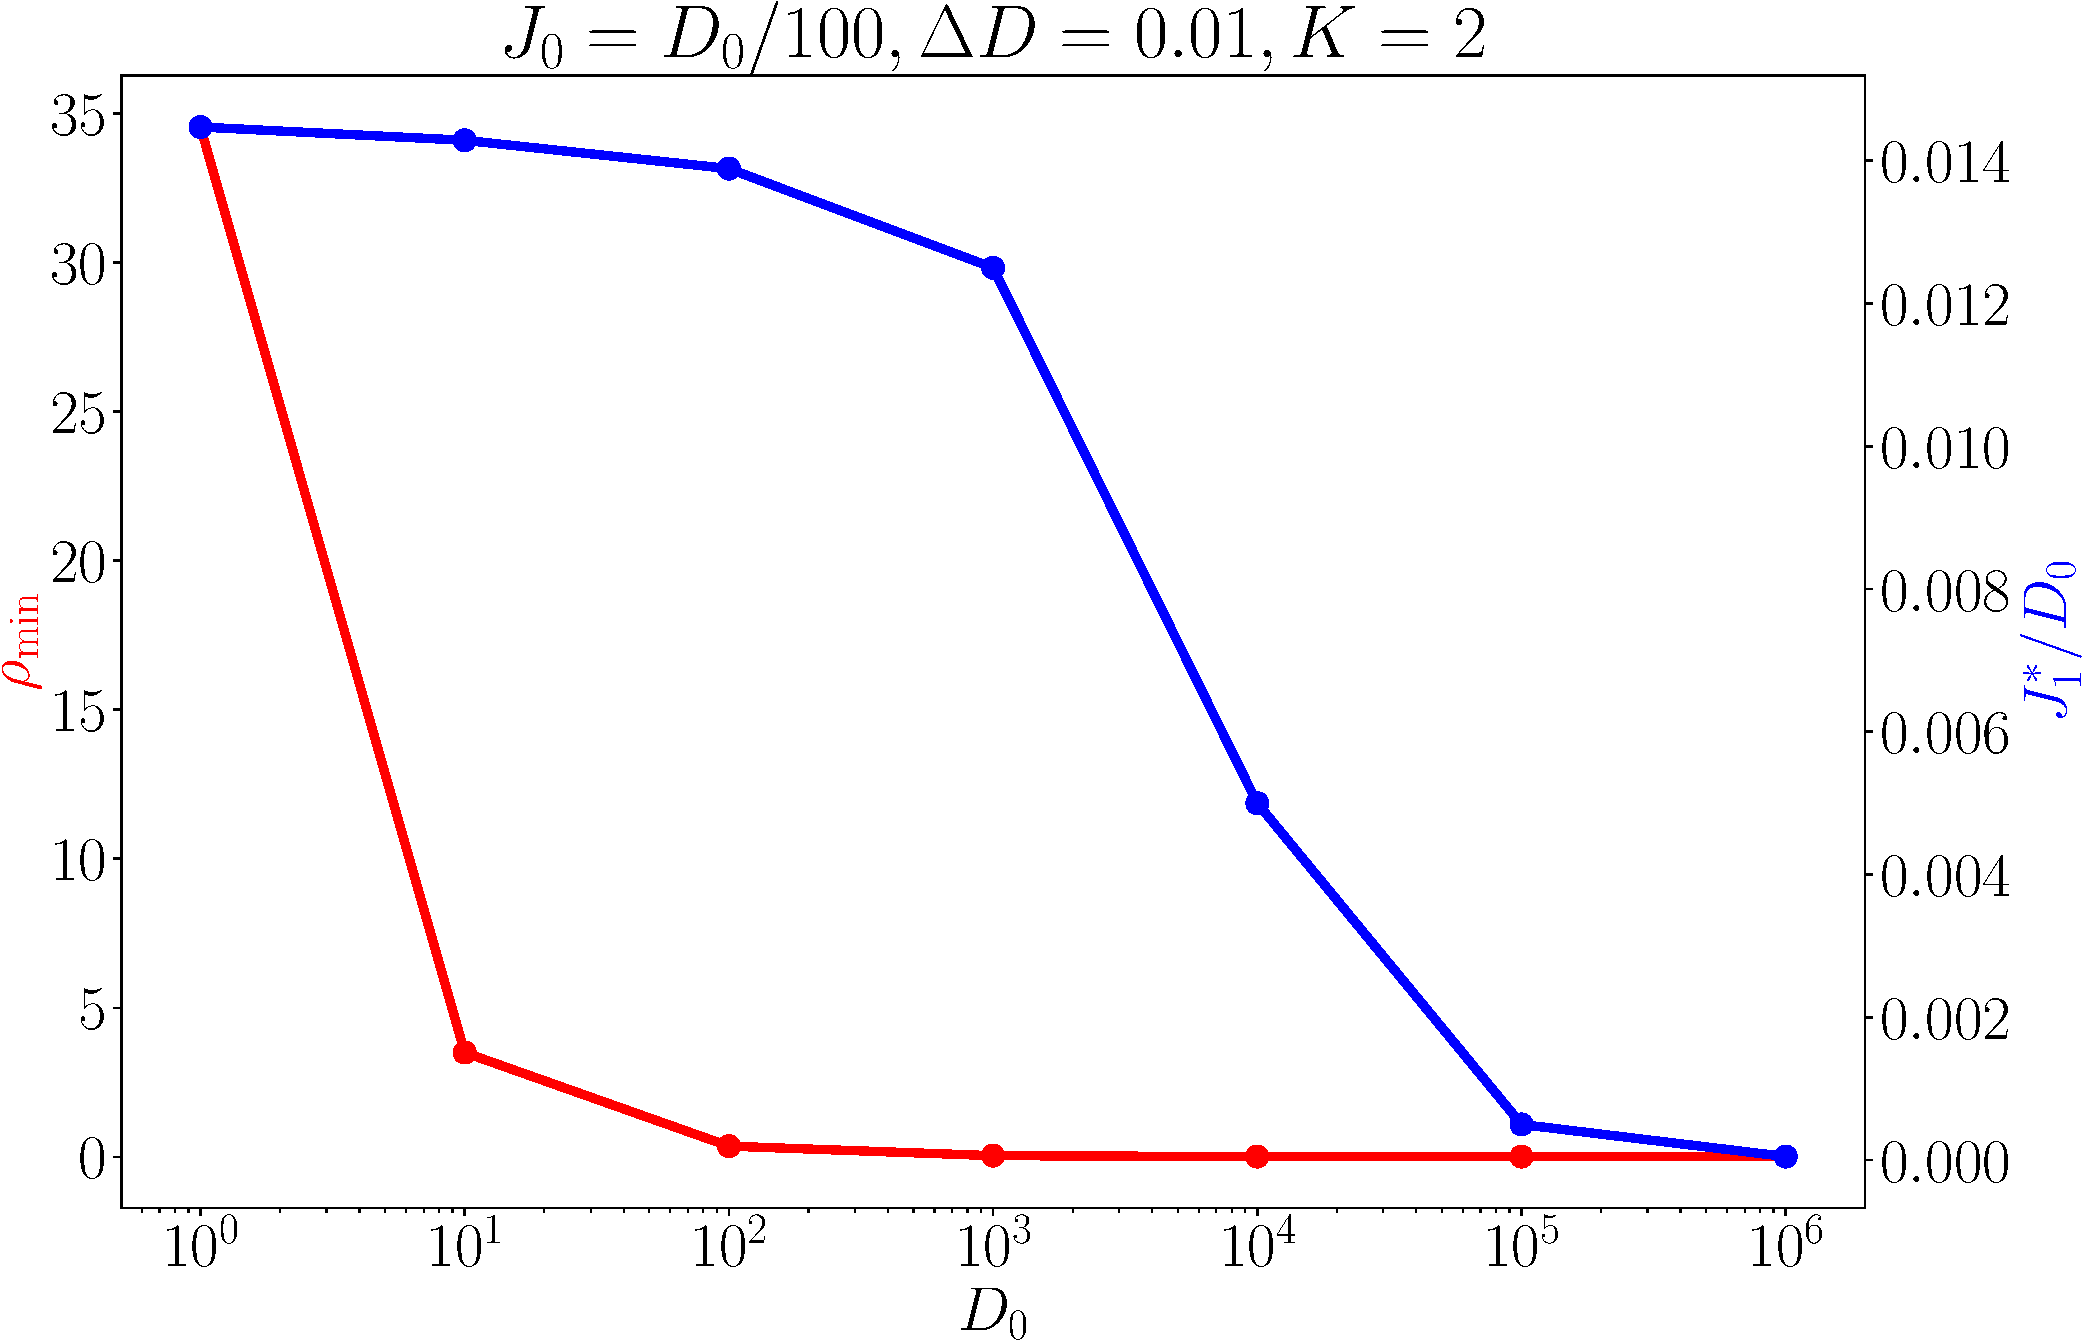
\includegraphics[width=0.7\textwidth]{./rhomin_D.pdf}
	\caption{Red curve shows variation of \(\rho_\text{min}\) against \(D_0\). It vanishes at large \(D_0\). Blue curve shows variation of the ratio \(J_1^* / D_0\) with \(D_0\). That shrinks as well, showing that the fixed point \(J_1^*\) remains finite in the thermodynamic limit, and the distance between \(J_1^*\) and \(J_2^*\) keeps growing.}
	\label{rhomin_vs_D}
\end{figure}

If we assume we are at a sufficiently large \(D_0\) and \(\rho > \rho_\text{min}\), the lower fixed point is \(J_1^*\). As shown in fig.~\ref{rhomin_vs_D}, we have \(J_1^* \ll D_0\). If we start with \(J_0\) in the neighborhood of \(J_1^*\), we can use \(J_1^* \ll D_0\) to ignore \(J\) in the denominator and the RG equation reduces to the poor man's scaling form eq.~\ref{pms_mchannel}. The denominator fixed point has effectively moved off to infinity. That this is true can also be argued from the single-channel Kondo model URG results. There, we saw that when the bandwidth is scaled to larger values, the strong-coupling fixed point was stable at successively larger values of \(J^*\). Since the denominator fixed point is identical in structure in both problems, its reasonable that the same thing will happen here.
